% This must be in the first 5 lines to tell arXiv to use pdfLaTeX, which is strongly recommended.
\pdfoutput=1
% In particular, the hyperref package requires pdfLaTeX in order to break URLs across lines.

\documentclass[11pt]{article}

% Change "review" to "final" to generate the final (sometimes called camera-ready) version.
% Change to "preprint" to generate a non-anonymous version with page numbers.
\usepackage[preprint]{coling}

% Standard package includes
\usepackage{times}
\usepackage{latexsym}

% For proper rendering and hyphenation of words containing Latin characters (including in bib files)
\usepackage[T1]{fontenc}
% For Vietnamese characters
% \usepackage[T5]{fontenc}
% See https://www.latex-project.org/help/documentation/encguide.pdf for other character sets

% This assumes your files are encoded as UTF8
\usepackage[utf8]{inputenc}

% This is not strictly necessary, and may be commented out,
% but it will improve the layout of the manuscript,
% and will typically save some space.
\usepackage{microtype}

% This is also not strictly necessary, and may be commented out.
% However, it will improve the aesthetics of text in
% the typewriter font.
\usepackage{inconsolata}

%Including images in your LaTeX document requires adding
%additional package(s)
\usepackage{graphicx}


\usepackage{tablefootnote}

% \usepackage[table,x11names]{xcolor}
\usepackage{color, colortbl}
\definecolor{verylightgray}{rgb}{0.9,0.9,0.9}
\definecolor{gray}{rgb}{0.5,0.5,0.5}
\definecolor{pygreen}{rgb}{0.0, 0.5, 0.0}
\definecolor{pyred}{rgb}{0.7, 0.0, 0.0}
\definecolor{pyblue}{rgb}{0.0, 0.0, 0.7}
\definecolor{pygray}{rgb}{0.5, 0.5, 0.5}
\definecolor{pydarkgray}{rgb}{0.3, 0.3, 0.3}

\definecolor{color1}{HTML}{006EB8}
\definecolor{color2}{HTML}{009B55}
\newcommand{\myblue}[1]{\textcolor{azureblue}{~#1}}
\newcommand{\myorange}[1]{\textcolor{orange}{~#1}}

\usepackage{wrapfig}

\usepackage[symbol]{footmisc}

\usepackage[T1]{fontenc}
\usepackage{multirow}
\usepackage{microtype}
\usepackage{hyperref}
\hypersetup{colorlinks=true,urlcolor=color2,linkcolor=color2,citecolor=color2}
\usepackage{url}
\usepackage{booktabs}
\usepackage{graphicx}
\usepackage{subcaption}
\usepackage[whole]{bxcjkjatype}
\usepackage{amsmath} 
\usepackage[inline]{enumitem}
% For Sonny's comment
\newcommand{\SVX}[1]{\textcolor{red}{[SVX: #1]}}
\newcommand{\Q}[1]{\textcolor{red}{[#1]}}


%% for non-anonymous version
% \newcommand{\system}{\textsc{Aurora-M}} 

% for submission
\newcommand{\system}{\textsc{Aurora-M}}


% If the title and author information does not fit in the area allocated, uncomment the following
%
%\setlength\titlebox{<dim>}
%
% and set <dim> to something 5cm or larger.

\title{\textsc{\system}: Open Source Continual Pre-training for Multilingual Language and Code}

% \title{\textsc{\system}: The First Open Source Multilingual Language Model Red-teamed according to the U.S. Executive Order}

% Author information can be set in various styles:
% For several authors from the same institution:
% \author{Author 1 \and ... \and Author n \\
%         Address line \\ ... \\ Address line}
% if the names do not fit well on one line use
%         Author 1 \\ {\bf Author 2} \\ ... \\ {\bf Author n} \\
% For authors from different institutions:
% \author{Author 1 \\ Address line \\  ... \\ Address line
%         \And  ... \And
%         Author n \\ Address line \\ ... \\ Address line}
% To start a separate ``row'' of authors use \AND, as in
% \author{Author 1 \\ Address line \\  ... \\ Address line
%         \AND
%         Author 2 \\ Address line \\ ... \\ Address line \And
%         Author 3 \\ Address line \\ ... \\ Address line}

% \author{First Author \\
%   Affiliation / Address line 1 \\
%   Affiliation / Address line 2 \\
%   Affiliation / Address line 3 \\
%   \texttt{email@domain} \\\And
%   Second Author \\
%   Affiliation / Address line 1 \\
%   Affiliation / Address line 2 \\
%   Affiliation / Address line 3 \\
%   \texttt{email@domain} \\}

% \author{
%    Aurora Team\\
%    Ontocord.AI
% }
\author{
Taishi Nakamura$^{*1}$, 
Mayank Mishra$^{*2}$, 
Simone Tedeschi$^{*3,4}$, 
Yekun Chai$^5$ \\
\textbf{Jason T Stillerman}, 
\textbf{Felix Friedrich}$^{6,7}$, 
\textbf{Prateek Yadav}$^8$, 
\textbf{Tanmay Laud}, \\
\textbf{Vu Minh Chien}$^9$, 
\textbf{Terry Yue Zhuo}$^{10,11}$, 
\textbf{Diganta Misra}$^{12,13}$, 
\textbf{Ben Bogin}$^{14}$, \\
\textbf{Xuan-Son Vu}$^{15,16,17}$, 
\textbf{Marzena Karpinska}$^{18}$, 
\textbf{Arnav Varma Dantuluri}, 
\textbf{Wojciech Kusa}$^{33}$, \\
\textbf{Tommaso Furlanello}, 
\textbf{Rio Yokota}$^1$, 
\textbf{Niklas Muennighoff}, 
\textbf{Suhas Pai}$^{19}$, \\
\textbf{Tosin Adewumi}$^{20}$, 
\textbf{Veronika Laippala}, 
\textbf{Xiaozhe Yao}$^{21}$, 
\textbf{Adalberto Junior}, \\
\textbf{Alpay Ariyak}$^{22,23}$, 
\textbf{Aleksandr Drozd}$^{24}$, 
\textbf{Jordan Clive}$^{25}$, 
\textbf{Kshitij Gupta}$^{12}$, \\
\textbf{Liangyu Chen}, 
\textbf{Qi Sun}$^1$, 
\textbf{Ken Tsui}, 
\textbf{Noah Persaud}, \\
\textbf{Nour Fahmy}, 
\textbf{Tianlong Chen}$^8$, 
\textbf{Mohit Bansal}$^8$, 
\textbf{Nicolò Monti}$^{26}$, \\
\textbf{Tai Dang}$^{18}$, 
\textbf{Ziyang Luo}$^{27}$, 
\textbf{Tien-Tung Bui}$^{28}$, 
\textbf{Roberto Navigli}$^3$, \\
\textbf{Virendra Mehta}$^{29}$, 
\textbf{Matthew Blumberg}$^{\#30}$, 
\textbf{Victor May}$^{\#31,32}$, 
\textbf{Huu Nguyen}$^{\#32}$, \\
\textbf{Sampo Pyysalo}$^{\#34}$ \\[1ex]
$^1$Institute of Science Tokyo,
$^2$MIT-IBM Watson Lab,
$^3$Sapienza University of Rome,\\
$^4$Babelscape,
$^5$LAION,
$^6$TU Darmstadt,
$^7$hessian.AI,
$^8$UNC Chapel-Hill \\
$^9$Detomo Inc.,
$^{10}$CSIRO's Data61,
$^{11}$Monash University,
$^{12}$Mila - Quebec AI Institute \\
$^{13}$Carnegie Mellon University,
$^{14}$Allen Institute for AI,
$^{15}$DeepTensor AB,\\
$^{16}$WASP Media \& Language,
$^{17}$Umeå University,
$^{18}$University of Massachusetts Amherst,\\
$^{19}$Hudson Labs,
$^{20}$Luleå University of Technology,
$^{21}$ETH Zurich,
$^{22}$RunPod,
$^{23}$OpenChat, \\
$^{24}$RIKEN CCS,
$^{25}$Chattermill AI,
$^{26}$ASC27,
$^{27}$Hong Kong Baptist University,
$^{28}$DopikAI JSC \\
$^{29}$University of Trento,
$^{30}$GridRepublic,
$^{31}$Chegg,
$^{32}$Ontocord.AI,
$^{33}$TU Wien,
$^{34}$University of Turku \\[1ex]
\texttt{taishi@rio.scrc.iir.isct.ac.jp},
\texttt{mayank.mishra2@ibm.com}, \\
\texttt{tedeschi@diag.uniroma1.it},
\texttt{praty@cs.unc.edu} \\
\texttt{diganta.misra@mila.quebec},
\texttt{mayvic@gmail.com}, \\
\texttt{s.vu@deeptensor.ai},
\texttt{huu@ontocord.ai},
\texttt{sampo.pyysalo@utu.fi} \\[1ex]
\texttt{\small $^*$Equal contribution \quad $^\#$Equal mentoring}
}
\vspace{10cm}


%\author{
%  \textbf{First Author\textsuperscript{1}},
%  \textbf{Second Author\textsuperscript{1,2}},
%  \textbf{Third T. Author\textsuperscript{1}},
%  \textbf{Fourth Author\textsuperscript{1}},
%\\
%  \textbf{Fifth Author\textsuperscript{1,2}},
%  \textbf{Sixth Author\textsuperscript{1}},
%  \textbf{Seventh Author\textsuperscript{1}},
%  \textbf{Eighth Author \textsuperscript{1,2,3,4}},
%\\
%  \textbf{Ninth Author\textsuperscript{1}},
%  \textbf{Tenth Author\textsuperscript{1}},
%  \textbf{Eleventh E. Author\textsuperscript{1,2,3,4,5}},
%  \textbf{Twelfth Author\textsuperscript{1}},
%\\
%  \textbf{Thirteenth Author\textsuperscript{3}},
%  \textbf{Fourteenth F. Author\textsuperscript{2,4}},
%  \textbf{Fifteenth Author\textsuperscript{1}},
%  \textbf{Sixteenth Author\textsuperscript{1}},
%\\
%  \textbf{Seventeenth S. Author\textsuperscript{4,5}},
%  \textbf{Eighteenth Author\textsuperscript{3,4}},
%  \textbf{Nineteenth N. Author\textsuperscript{2,5}},
%  \textbf{Twentieth Author\textsuperscript{1}}
%\\
%\\
%  \textsuperscript{1}Affiliation 1,
%  \textsuperscript{2}Affiliation 2,
%  \textsuperscript{3}Affiliation 3,
%  \textsuperscript{4}Affiliation 4,
%  \textsuperscript{5}Affiliation 5
%\\
%  \small{
%    \textbf{Correspondence:} \href{mailto:email@domain}{email@domain}
%  }
%}

\begin{document}
\setlength\titlebox{35\baselineskip}
\maketitle
\begin{abstract}
Pretrained language models are an integral part of AI applications, but their high computational cost for training limits accessibility. 
Initiatives such as \textsc{Bloom} and \textsc{StarCoder} aim to democratize access to pretrained models for collaborative community development. 
Despite these efforts, such models encounter challenges such as limited multilingual capabilities, risks of catastrophic forgetting during continual pretraining, and the high costs of training models from scratch, alongside the need to align with AI safety standards and regulatory frameworks.
%However, existing models face challenges: limited multilingual capabilities, continual pretraining causing catastrophic forgetting whereas pretraining from scratch is computationally expensive, and compliance with AI safety and development laws. 
%
This paper presents \textbf{\textcolor{violet}{\system}}, a \texttt{15B} parameter multilingual open-source model trained on English, Finnish, Hindi, Japanese, Vietnamese, and code. Continually pretrained from \textsc{StarCoderPlus} on \texttt{435B} additional tokens, \system\ surpasses \texttt{2T} tokens in total training token count. It is the first open-source multilingual model fine-tuned on human-reviewed safety instructions, thus aligning its development not only with conventional red-teaming considerations, but also with the specific concerns articulated in the Biden-Harris Executive Order on the Safe, Secure, and Trustworthy Development and Use of Artificial Intelligence.
%
We evaluate \system\ across a wide range of tasks and languages, showcasing its robustness against catastrophic forgetting and its superior performance in multilingual settings, particularly in safety evaluations. We open-source \system\ and its variants to encourage responsible open-source development of large language models at \url{https://huggingface.co/aurora-m}.

% \begin{center}
%    % 
\includegraphics[width=0.03\textwidth]{img/huggingface_logo_svg-tex.pdf}
%    \url{https://huggingface.co/aurora-m}
% \end{center}
\end{abstract}

% To encourage responsible open-source development of large language models, \system\ and its variants are available at \url{https://huggingface.co/aurora-m}.
% \system\ is rigorously evaluated across various tasks and languages, demonstrating robustness against catastrophic forgetting and outperforming alternatives in multilingual settings, particularly in safety evaluations. To promote responsible open-source LLM development, \system\ and its variants are released at \url{https://huggingface.co/aurora-m}.
% \href{https://huggingface.co/collections/aurora-m/aurora-m-models-65fdfdff62471e09812f5407}{here}.
% \system\ is rigorously evaluated across various tasks and languages, demonstrating robustness against catastrophic forgetting and outperforming alternatives in multilingual settings, particularly in safety evaluations. To promote responsible open-source LLM development, \system\ and its variants will be made publicly available. 



\section{Introduction}
\section{Introduction}
Despite the well-recognized importance of training data in advancing the capabilities of large language models (LLMs)~\cite{brown2020language,kaplan2020scaling,Razeghi2022ImpactOP}, there is no agreed-upon mechanisms for crediting or compensating data providers. As LLMs are increasingly integrated into our society and economy, the absence of such mechanisms has aggravated a tension between data and model providers, exemplified by recent legal challenges involving major tech companies~\cite{jlversusalphabet,metz2022lawsuit}. In this atmosphere, data valuation, which quantifies the contribution of each training data to the model output, has been discussed as a potential technical solution for tackling these societal issues~\cite{fernandez2023data,ghorbani2019data,huang2023citation,jia2019towards,worledge2023unifying,zhao2023addressing}. 

At a high level, most data valuation algorithms interpret the model output as a coalition of its training data, and evaluate the contribution of each example based on its influence on the model output when included or excluded from the training dataset~\cite{ghorbani2019data,ilyas2022datamodels,koh2017understanding,kwon2021beta}. If an inclusion of a specific training example consistently improves model performance, high value can be assigned to this example for its contribution. However, applying existing data valuation methods to recent LLMs and their vast training datasets has faced significant scalability challenges to date. For instance, sampling-based methods, such as the Shapley value~\cite{ghorbani2019data,kwon2021beta} or Datamodels~\cite{ilyas2022datamodels}, require retraining the model multiple times with varied combinations of data subsets to directly model the effect of in/excluding each data. Unfortunately, such repeated retraining is hardly affordable even for small models, let alone LLMs. To overcome this issue, gradient-based methods, including influence functions~\cite{koh2017understanding,park2023trak}, approximate the effect of data in/exclusion on the model output using gradient information without costly retraining. Even so, scaling gradient-based methods to LLMs is hindered by prohibitive compute and memory costs originating in the high-dimensional nature of the gradient.

Consequently, the main objective of this work is to bridge the gap in scaling existing data valuation methods to recent LLMs and their vast training datasets. Toward this goal, we focus on influence functions \cite{koh2017understanding,park2023trak}, a representative gradient-based data valuation method, and significantly improve its scalability with an efficient gradient projection algorithm. We visualize the proposed data valuation system in Figure~\ref{fig:diagram}, and detail our technical contributions below:

\begin{figure}
    \centering
    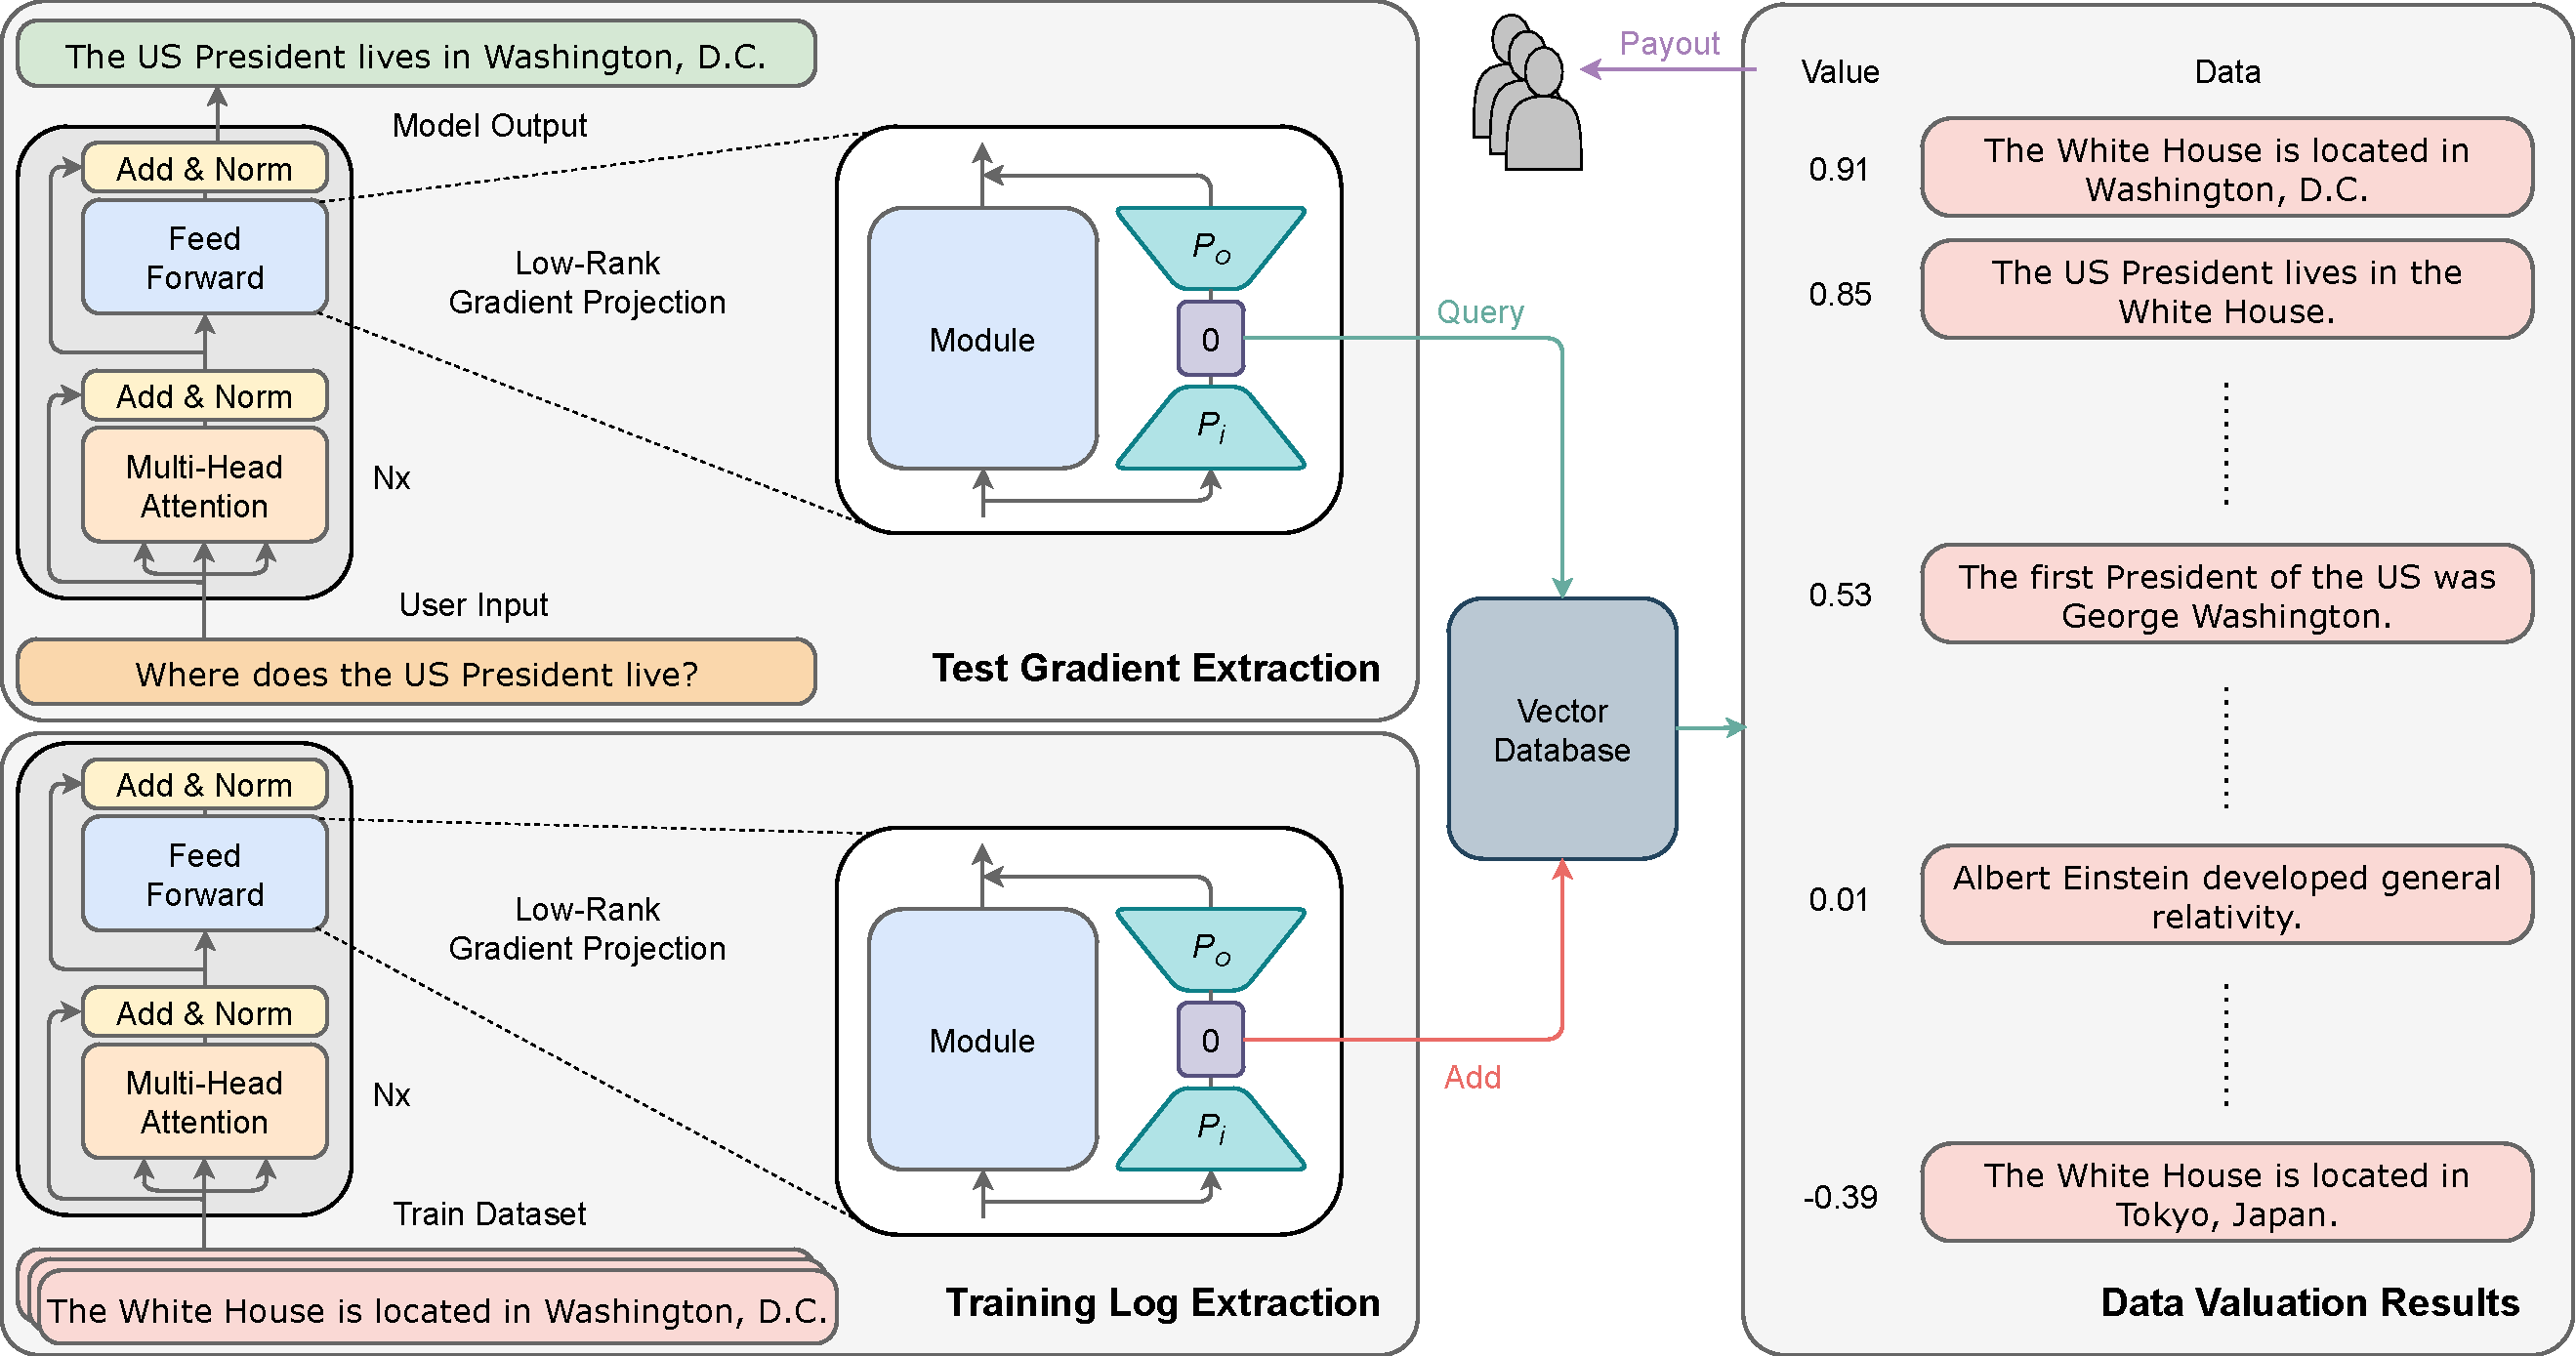
\includegraphics[width=0.94\textwidth]{figures/diagram_v7.pdf}
    \vskip -4pt
    \caption{Data valuation system architecture. \textbf{(Left Bottom)} We first extract the Hessian and gradients for all training data using efficient gradient projection \method\ and store them in a database. \textbf{(Left Top)} At test time, we similarly extract gradients and query the database. \textbf{(Right)} The database returns similarity scores with respect to training examples that can be used for data valuation/attribution.}
    \label{fig:diagram}
\end{figure}

\begin{itemize}[leftmargin=*,topsep=-2pt]
    \item Employing gradient structures in backpropagation, we develop a novel \textbf{lo}w-rank \textbf{gra}dient projection algorithm \method\ that improves space \& time complexity of gradient projection, a major scalability bottleneck in prior work~\cite{park2023trak,schioppa2022scaling}, from $O(nk)$ to $O(\sqrt{nk})$ where $n$ and $k$ are model and projection dimensions. Furthermore, \method\ directly computes projected gradients without materializing full gradients, enabling low GPU memory and high GPU utilization for improved efficiency. Lastly, we show that \method\ can be easily implemented with small add-on layers, similarly to LoRA~\cite{hu2021lora}.
    \item By interpreting a damping term in influence functions as a spectral gradient sparsification mechanism, we (1) offer a theoretical motivation of gradient projection approaches to influence functions and (2) derive a specialized PCA initialization scheme for \method.
    \item We introduce software named \software\ that (1) makes it \textit{simple} to convert existing training code into data valuation code, (2) is \textit{compatible} with various scalability tools and features in the LLM ecosystem, and (3) is \textit{extensible} to implement other data valuation or interpretability algorithms.
    \item In our data valuation experiments, \method\ demonstrates competitive accuracy against more costly baselines, while showing up to 6,500$\times$ increase in throughput and 5$\times$ reduction in GPU memory, when applied to Llama3-8B-Instruct~\cite{llama3modelcard} and the 1B-token dataset, compared to EKFAC influence \cite{grosse2023studying}, the state-of-the-art and only runnable baseline at this scale. We also observe that most valuable data identified by \method\ generally share qualitative similarities with the queried LLM output.
\end{itemize}

\section{Datasets}

\section{Text and Multi-modal Datasets}\label{sec:dataset}


In this section, we introduce the text and multi-modal datasets used to evaluate LLM efficiency.

\subsection{Text Dataset}\label{ssec:text_dataset}

% Text dataset, as the most commonly seen datasets involved in LLM's training, validation and testing, has diverged into many different tasks.
% We summarized some long-context datasets that was adapted and used in state-of-the-art benchmark frameworks, namely \textbf{L-Eval}~\cite{an_l-eval:_2023}, 
% \textbf{M4LE}~\cite{kwan_m4le:_2023}, \textbf{BAMBOO}~\cite{dong2023bamboo}, \textbf{LongBench}~\cite{bai_longbench:_2023}, \textbf{LRA}~\cite{tay_long_lra_2020}, 
% \textbf{SCORLLS}~\cite{shaham_scrolls:_2022}, \textbf{ZEROSCROLLS}~\cite{shaham_zeroscrolls:_2023}  \textbf{LooGLE}~\cite{li_loogle:_2023}, \textbf{LongEval}~\cite{longchat2023}  and \textbf{StreamingEval}~\cite{DBLP:conf/iclr/XiaoTCHL24}.  
% We do our survey at dataset level, and looked into the original dataset for more detailed information.  \ref{tab:text-dataset-qa}, \ref{tab:text-dataset-summarization}, \ref{tab:text-dataset-nli-classification}, \ref{tab:text-dataset-generation}, \ref{tab:text-dataset-retrieval}, \ref{tab:text-dataset-aggregation} describe datasets that are ready-to-use, or have a large text resource to build new datasets with. In all, the tasks text datasets apply to can be categorized into the following types:

We collect a lot of long-context datasets from state-of-the-art benchmark frameworks and various papers, including L-Eval\cite{an_l-eval:_2023}, M4LE\cite{kwan_m4le:_2023}, BAMBOO\cite{dong2023bamboo}, LongBench\cite{bai_longbench:_2023}, LRA\cite{tay_long_lra_2020}, SCROLLS\cite{shaham_scrolls:_2022}, ZEROSCROLLS\cite{shaham_zeroscrolls:_2023}, LooGLE\cite{li_loogle:_2023}, LongEval\cite{longchat2023}, and StreamingEval\cite{DBLP:conf/iclr/XiaoTCHL24}.
Specifically,
we categorize these datasets into different tasks, including question answering, text summarization, text reasoning, text retrieval, and text generation.

%Text-QA
\begin{table*}[t]
    \centering
    \caption{Text question answering (QA) dataset. In the \textbf{Avg. Len: }  average length, \textbf{Tok:}  tokens;  \textbf{W: } words. In the Instances column, \textbf{Doc:} documents, \textbf{Q:} questions, \textbf{Inst:} instructions. Particularly, AltQA, PaperQA and MeetingQA have two datasets  with different length levels, and is separated with $/$. \\
    %In the Metric column, \textbf{EM:} Exact Match. \textbf{Acc:} Accuracy. \textbf{METEOR}~\cite{denkowski-lavie-2011-meteor} is a machine translation evaluation metric that incorporates factors like stemming, synonym matching, and word order to provide a more nuanced assessment of translation quality. 
    %\textbf{BLEU}\cite{papineni-etal-2002-bleu} is also a metric designed for machine translation. 
    %\textbf{Rouge}~\cite{lin-2004-rouge} and its variants measure model's performance by calculating overlap between model output and reference answer with unigram(Rouge-1), bigram(Rouge-2), LCS(Rouge-L), etc.  
    %\textbf{F1}~\cite{rajpurkar-etal-2016-squad-F1} calculates unigram overlap between model output and answers after processing elments like white-spaces and stop-words. 
    Particularly, for datasets from L-Eval, the GPT-4 metric means the win-rate against Turbo-16K, judged by GPT-4. $\Delta L$ is the length difference between answer length and ground truth. For NarrativeQA, \textbf{MRR: }Mean Reciprocal Rank .} 
    \renewcommand{\arraystretch}{1.5} % 调整行间距
    \setlength{\tabcolsep}{1pt} % 减小列间距
    \label{tab:text-dataset-qa}
\begin{tabular}{c|c|c|c|c|c|c}
\hline
\textbf{Task} &
  \textbf{Name} &
  \textbf{Source} &
  \textbf{Instances} &
  \textbf{Avg Len} &
  \textbf{Metric} &
  \textbf{Lang.} \\ \hline
QA &
  \href{https://github.com/abacusai/long-context}{AltQA}~\cite{pal2023giraffeadventuresexpandingcontext} &
  Wikipedia &
  200/200 &
  3243/13,084 Tok&
  Acc &
  EN \\ \hline

QA &
  \href{https://github.com/RUCAIBox/BAMBOO/tree/main/datasets}{PaperQA(BAMBOO)}~\cite{dong2023bamboo} &
  Paper &
  100/100 &
  3101/6838 Tok&
  Acc &
  EN \\ \hline

QA &
  \href{https://github.com/RUCAIBox/BAMBOO/tree/main/datasets}{MeetingQA(BAMBOO}~\cite{dong2023bamboo}  &
  Meeting &
  100/100 &
  2738/9838 Tok&
  Acc &
  EN \\ \hline



QA &
  \href{https://huggingface.co/datasets/mandarjoshi/trivia_qa}{TriviaQA}~\cite{joshi_triviaqa:_2017}  &
  Web Question, Wiki &
  95,956 Q, 662,659 Doc&
  17,370 W&
  EM, F1 &
  EN \\ \hline



QA&
  \href{https://github.com/OpenLMLab/LEval}{TOEFL(L-Eval)}~\cite{an_l-eval:_2023} &
  TOFEL-QA\cite{tseng_towards_tofelqa_2016} &
  15 Doc, 269 Inst&
  3907 Tok&
   Rouge-L, GPT-4, $\Delta L$&
  EN \\ \hline


QA&
   \href{https://github.com/OpenLMLab/LEval}{Coursera(L-Eval)}~\cite{an_l-eval:_2023} &
  Video Subtitles&
  15 Doc, 172 Inst&
  9075 Tok&
   Rouge-L, GPT-4, $\Delta L$&
  EN \\ \hline


QA &
   \href{https://github.com/OpenLMLab/LEval}{SFiction(L-Eval)}~\cite{an_l-eval:_2023} &
  SFGram \cite{sfgram}, fiction&
  7 Doc, 64 Inst&
  16,381 Tok&
   Rouge-L, GPT-4, $\Delta L$&
  EN \\ \hline


QA &
   \href{https://github.com/OpenLMLab/LEval}{LongFQA(L-Eval)}~\cite{an_l-eval:_2023} &
  Financial Transcripts&
  6 Doc, 52 Inst&
  6032 Tok&
   Rouge-L, GPT-4, $\Delta L$&
  EN \\ \hline

QA &
   \href{https://github.com/OpenLMLab/LEval}{CUAD(L-Eval)}~\cite{an_l-eval:_2023} &
  CUAD\cite{hendrycks_cuad:_2021} &
  20 Doc, 130 Inst&
  30,966 Tok&
   Rouge-L, GPT-4, $\Delta L$&
  EN \\ \hline


QA &
  \href{https://github.com/KwanWaiChung/M4LE}DuoRC~\cite{kwan_m4le:_2023} &
  Movie &
   &
  3572 W&
  Acc &
  EN \\ \hline


QA &
  \href{https://ai.google.com/research/NaturalQuestions/download}{NQ~\cite{kwiatkowski_nq_2019}}&
  Wiki &
  307,373 &
  9005 W &
  Rouge &
  EN \\ \hline


  
QA-SG&
  \href{https://github.com/google-deepmind/narrativeqa}{NarrativeQA}~\cite{narrativeqa}  &
  Story &
  1572 Doc&
  62,528 Tok&
  \begin{tabular}[c]{@{}c@{}}BLEU, METEOR, \\ Rouge-L, MRR\end{tabular}&
  EN \\ \hline

QA-SG &
  \href{https://huggingface.co/datasets/THUDM/LongBench}{NarrativeQA(LongBench)}~\cite{bai_longbench:_2023} &
  Story &
  200 &
  18,409 W &
  F1 &
  EN \\ \hline

QA-SG&
  \href{https://huggingface.co/datasets/allenai/qasper}{Qasper}~\cite{dasigi_dataset_2021_qasper} &
  Paper &
  1585 &
  5001 W&
  F1 &
  EN \\ \hline

QA-SG &
  \href{https://huggingface.co/datasets/THUDM/LongBench}{Qasper(LongBench)}~\cite{bai_longbench:_2023}  &
  Paper &
  200 &
  3619 W&
  F1 &
  EN \\ \hline

QA-SG&
  \href{https://huggingface.co/datasets/THUDM/LongBench}{MultifieldQA-en}~\cite{bai_longbench:_2023}  &
  \begin{tabular}[c]{@{}c@{}}Paper, Legal, \\ Gov, Google\end{tabular}&
  200 &
  4459 W&
  F1 &
  EN \\ \hline

QA-SG&
  \href{https://huggingface.co/datasets/THUDM/LongBench}{MultifieldQA-zh}~\cite{yang_hotpotqa:_2018} &
\begin{tabular}[c]{@{}c@{}}Paper, Legal, \\ Gov, Google\end{tabular}&
  200 &
  6701 W&
  F1 &
  ZH \\ \hline


  QA-SG &
  \href{https://github.com/nyu-mll/quality}{QuALITY}~\cite{pang_quality_dataset:_2021} &
  Story, magazine&
  381 Doc, 6737 Q&
  4203 W&
  EM &
  EN \\ \hline


  
QA-MT&
  \href{https://huggingface.co/datasets/hotpotqa/hotpot_qa}{HotpotQA}~\cite{yang_hotpotqa:_2018} &
  Wiki &
  112,779 &
  1138 W&
  EM, F1 &
  EN \\ \hline


QA-MT&
  \href{https://huggingface.co/datasets/THUDM/LongBench}{HotpotQA(LongBench)}~\cite{bai_longbench:_2023} &
  Wiki &
  200 &
  9151 W&
  F1 &
  EN \\ \hline


QA-MT&
  \href{https://github.com/Alab-NII/2wikimultihop}{2WikiMultihopQA}~\cite{ho_multihopqa_2020} &
  Wiki &
  192,606 Q&
  639 W&
  EM, F1 &
  EN \\ \hline


QA-MT&
  \href{https://github.com/stonybrooknlp/musique}{MuSiQue}~\cite{trivedi_musique:_2021} &
  Wiki &
  24,814 &
  1827 W&
  F1 &
  EN \\ \hline

QA-MT&
  \href{https://github.com/baidu/DuReader}{DuReader}~\cite{he_dureader:_2017} &
  Baidu &
  200,000 Q, 1,000,000 Doc&
  396 W&
  BLEU, Rouge-L &
  ZH,EN \\ \hline
  
QA+RET &
  \href{https://github.com/KwanWaiChung/M4LE}{NewsQA(M4LE)}~\cite{kwan_m4le:_2023} &
  News &
  - &
  3679 W&
  Acc &
  EN \\ \hline

QA+RET &
  \href{https://github.com/KwanWaiChung/M4LE}{C3(M4LE)}~\cite{kwan_m4le:_2023} &
  Textbook&
  - &
  3797 W&
  Acc &
  ZH \\




 \hline
\end{tabular}
\end{table*}



\subsubsection{Question Answering (QA) Task}
Dataset for this task usually consist of question-answer pairs, and documents that contains the answer to the question. For a model to run such task, documents and questions are usually used as the model input, while the output can differ greatly. Some datasets' answers are closed-ended, meaning that the model should only output its answer in designated form, typically multiple choice answers, while the open-ended answers take a more free form. According to the number of documents involved in a question-answer pair, we can categorize QA task datasets into single-doc QA(QA-SG) and multiple-doc QA(QA-MT). The detailed statistics of the datasets for question answering are provided in Table~\ref{tab:text-dataset-qa}.


%Text-SUM
\begin{table*}[]
    \centering
    \caption{Text Dataset-Summarization. In the \textbf{Avg. Len: }  average length, \textbf{Tok:}  tokens;  \textbf{W: } words. In the Instances column, \textbf{Doc:} documents, \textbf{Q:} questions, \textbf{Inst:} instructions. Particularly, SPACE has the concept of 'Entity', and R/Ent stands for reviews per entity. Sum stands for summary.  
    In the Metric column, \textbf{EM:} Exact Match. \textbf{PM:} Partial Match. \textbf{Acc:} Accuracy. 
    %\textbf{METEOR}~\cite{denkowski-lavie-2011-meteor} and \textbf{BLEU}\cite{papineni-etal-2002-bleu} are a machine translation evaluation metric.
    %that incorporates factors like stemming, synonym matching, and word order to provide a more nuanced assessment of translation quality. 
    %\textbf{BLEU}\cite{papineni-etal-2002-bleu} is also a metric designed for machine translation. 
    %\textbf{Rouge}~\cite{lin-2004-rouge} measures model's performance with the ngram overlap between model output and reference answer. \textbf{F1}~\cite{rajpurkar-etal-2016-squad-F1} calculates unigram overlap between model output and answers after processing elments like white-spaces and stop-words. 
    %\textbf{BERT}~\cite{zhang2020bertscoreevaluatingtextgeneration} is a text generation task metric using contextual embeddings. 
    For MultiNews, \textbf{Rouge-SU} skip bigrams when having a distance larger than 4 words. Particularly, LooGLE utilizes GPT-4 for its QA and summarization task, using it for answer's semantic judgement.}
    \renewcommand{\arraystretch}{1.3} % 调整行间距
    \setlength{\tabcolsep}{1pt} % 减小列间距
    \label{tab:text-dataset-summarization}

\begin{tabular}{c|c|c|c|c|c|c}
\hline
\textbf{Task} &
  \textbf{Name} &
  \textbf{Source} &
  \textbf{Instances} &
  \textbf{Avg Len} &
  \textbf{Metric} &
  \textbf{Lang.} \\ \hline
 SUM& 
\href{https://huggingface.co/datasets/ccdv/cnn_dailymail}{CNN/Dailymail}~\cite{nallapati_abstractive_dailymail_2016}& News& 
300,000& 
766 W& 
Rouge-1/2/L&
EN\\ \hline
 SUM
 & \href{https://huggingface.co/datasets/EdinburghNLP/xsum}{XSum}~\cite{narayan_dont_xsum_2018}
 & News
 & 400,000
 & 431 W
 & Rouge-1/2/L
 &EN\\ \hline
 SUM
 & \href{https://github.com/Yale-LILY/QMSum}{QMSum}~\cite{zhong_qmsum:_2021}
 & Meeting
 & 232 Meets, 1808 Q
 & 9070 W
 & Rouge-1/2/L
 &EN\\  \hline
 SUM
 & \href{https://github.com/Alex-Fabbri/Multi-News}{MultiNews}~\cite{fabbri_multi-news:_2019}
 & News
 & 51,216
 & 5866 W %2103.49*2.788
 & Rouge-1/2/SU
 &EN\\ \hline
 
\begin{tabular}[c]{@{}c@{}}SUM-QB+\\Reasoning+\\QA\end{tabular}& %Note: also support Cloze task 
  \href{https://github.com/bigai-nlco/LooGLE}{LooGLE}~\cite{li_loogle:_2023} &
  \begin{tabular}[c]{@{}c@{}}Papers, Wiki,\\ Movie, TV \end{tabular}&
  776 Doc, 6448 Q&
  \begin{tabular}[c]{@{}c@{}}19,367 W\\24,005 Tok\end{tabular}&
  \begin{tabular}[c]{@{}c@{}}BLEU, Rouge, METEOR, \\BERT, GPT4, \\EM, PM \end{tabular}&
  EN,ZH \\ \hline

SUM &
  \href{https://huggingface.co/datasets/ccdv/govreport-summarization}{GovReport}~\cite{huang_govreport_2021} &
  Gov &
  19,466 &
  \begin{tabular}[c]{@{}c@{}}9409.4 W\end{tabular}&
  Rouge-1/2/L&
  EN \\ \hline
SUM &
  \href{https://github.com/hahahawu/VCSum}{VCSUM}~\cite{wu_vcsum:_2023} &
  Meeting &
  239 &
  14,107 Tok&
  F1, Gold Rouge-1&
  ZH \\ \hline
%SUM &
%  \href{https://arxiv.org/src/1911.12237v2/anc}{SAMSum}~\cite{gliwa_samsum_2019} &
%  Dialogue &
%  16,369 &
%  109 W &
%  Rouge&
%  EN \\ \hline
SUM &
  \href{https://github.com/mingdachen/SummScreen}{SummScreenFD}~\cite{chen_summscreen:_2021} &
  TV &
  269,000 &
  6613 Tok&
  Rouge&
  EN \\ \hline

SUM &
  \href{https://evasharma.github.io/bigpatent/}{BigPatent}~\cite{sharma_bigpatent:_2019} &
  Patent &
  1,341,362 &
  3573 W&
  Rouge-1/2/L&
  EN \\ \hline
SUM &
  \href{https://github.com/stangelid/qt}{SPACE}~\cite{angelidis_extractive_space_2021} &
  Review&
  \begin{tabular}[c]{@{}c@{}}50 Entities, \\1,140,000 Reviews, \\100R/Ent, \\1050 Sum\end{tabular}&
  15,532 W &
  Rouge-1/2/L&
  EN \\ \hline
SUM &
  \href{https://github.com/nyu-mll/SQuALITY}{SQuALITY} ~\cite{wang2022squality}&
  Story&
  625&
  \begin{tabular}[c]{@{}c@{}}5200 W\end{tabular}&
  \begin{tabular}[c]{@{}c@{}}Rouge-1/2/L, \\METEOR, \\BERT\end{tabular}&
  EN \\ \hline
SUM+RET &
  \href{https://github.com/KwanWaiChung/M4LE}{CNNNews(M4LE)}~\cite{kwan_m4le:_2023} &
  News &
  - &
  3754 W &
  Rouge-L &
  EN \\ \hline
SUM+RET &
  \href{https://github.com/KwanWaiChung/M4LE}{CEPSUM(M4LE)}~\cite{kwan_m4le:_2023} &
  E-Commerce &
  - &
  4003 W &
  Rouge-L & 
  ZH \\  \hline
SUM+RET &
  \href{https://github.com/KwanWaiChung/M4LE}{LCSTS(M4LE)}~\cite{kwan_m4le:_2023} &
  News &
  - &
  4102 W &
  Rouge-L &
  ZH \\ \hline
SUM+RET &
  \href{https://github.com/KwanWaiChung/M4LE}{NCLS(M4LE)}~\cite{kwan_m4le:_2023} &
  NCLS~\cite{zhu_ncls:_2019} &
  - &
  3470 W&
  Rouge-L &
  EN,ZH \\ \hline
SUM+RET &
  \href{https://github.com/KwanWaiChung/M4LE}{WikiHow}~\cite{kwan_m4le:_2023} &
  Wiki &
  - &
  3514 W &
  Rouge-L &
  EN \\ \hline
SUM+RET &
  \href{https://github.com/KwanWaiChung/M4LE}{News2016}~\cite{kwan_m4le:_2023} &
  News &
  - &
  3785 W &
  Rouge-L &
  ZH \\ \hline

SUM &
  \href{https://github.com/KwanWaiChung/M4LE}{Pubmed(M4LE)}~\cite{kwan_m4le:_2023} &
  Medical &
  1267 &
  3678 W &
  Rouge-L &
  EN \\ \hline
SUM &
  \href{https://github.com/KwanWaiChung/M4LE}{BookSum(M4LE)}~\cite{kwan_m4le:_2023} &
  Book &
  - &
  2643 W &
  Rouge-L &
  EN \\ \hline
SUM &
  \href{https://github.com/KwanWaiChung/M4LE}{CNewsum(M4LE)}~\cite{kwan_m4le:_2023} &
  News &
  690 &
  1883 W &
  Rouge-L &
  ZH \\ \hline
SUM &
  \href{https://github.com/KwanWaiChung/M4LE}{CLTS+(M4LE)}~\cite{kwan_m4le:_2023} &
  News &
  - &
  3158 W &
  Rouge-L &
  ZH \\ \hline
SUM &
  \href{https://github.com/KwanWaiChung/M4LE}{Arxiv(M4LE)}~\cite{kwan_m4le:_2023} &
  Paper&
  1550 &
  3748 W &
  Rouge-L &
  EN \\ \hline


 
\end{tabular}
\end{table*}

\begin{itemize}[leftmargin=10pt]
    \item \textbf{Qasper~\cite{dasigi_dataset_2021_qasper}} consists of 5049 questions based on 1585 papers on NLP.  Question is from NLP practitioners that only have read the abstract and title of a paper, then another set of practitioners answer these questions by reading through the whole paper. The supporting evidences is provided correspondingly. Each instance of the dataset consists of a question, an answer, corresponding paper and supporting evidence. Instances built by LongBench~\cite{bai_longbench:_2023} doesn't require evidence. 
    \item  \textbf{HotpotQA~\cite{yang_hotpotqa:_2018} } is a typical for a multi-doc QA dataset. It's built based on Wikipedia, and each instance consists of multiple documents, a question, an answer and supporting facts. Supporting facts is a set of paragraph indexes, annotated manually. 
    \item \textbf{AltQA~\cite{pal2023giraffeadventuresexpandingcontext}} is based on google's NQ~\cite{kwiatkowski_nq_2019} dataset. The answer are all numerical. The original document is "altered" so that each occurrences of the numerical answer is different from the original document, so as to avoid data contamination from pretraining. This dataset is also used in BAMBOO~\cite{dong2023bamboo} benchmark.
    \item \textbf{PaperQA} and \textbf{MeetingQA} from BAMBOO~\cite{dong2023bamboo} benchmark are question answering tasks in the form of multiple-choice.  Each instance of the two datasets consists of question , evidence, answer and corresponding content.
    \item \textbf{NarrativeQA}~\cite{narrativeqa} uses complex narratives that are self-contained as input documents. Both books and movie scripts are used. For question construction, annotators are only given a story summary, and are asked to write questions based on it. For each story(1572 stories in total), about 30 question-answer pairs are constructed from each summary-story pair. Notably, because of the consistency in story context, the task can be simplified to selecting a correct answer from all answers that relates to the story. 
    \item \textbf{MultifieldQA}~\cite{bai_longbench:_2023} is an original dataset from Longbench. Its contents covers scientific papers, legal documents, government reports and google results. The dataset has both Chinese and English version, and each instance consists of context built on documents, and a question-answer pair. 
    \item \textbf{2WikiMultihopQA}~\cite{ho_multihopqa_2020} is a multi-document QA dataset built on Wikipedia and Wikidata. WikiData is a Knowledge Graph database, from which the author was able to extract the (subject entity, property, object entity) triple that corresponds to a Wikipidia document. These triples are used as evidences in each QA pair, as a way for model to show its inference process. The dataset consists of 192,606 questions in total.
    \item \textbf{Musique~\cite{trivedi_musique:_2021}} is also a multi-document dataset(or multi-hop dataset, as the paper refers to). Its data is extracted from existing single-hop QA datasets. These single-hop QAs are then composed into multi-hop QA pairs. In addition, Musique add some unanswerable QA pairs in order to further test model's ability. There are 24,814 answerable questions in Musique, and each answerable question corresponds to an unanswerable question.
    \item \textbf{DuReader}~\cite{he_dureader:_2017} is a multi-document QA dataset, whose data is based on Baidu search results. It consists of 200,000 questions, 1,000,000 documents and 420,000 answers. Each instance contains a question, multiple possible answers(also possible to be empty), and multiple documents. 
    \item \textbf{TriviaQA}~\cite{joshi_triviaqa:_2017 } is a multi-document reading comprehension QA dataset. All QA pairs are from 14 trivia websites, written by trivia enthusiasts.  For each QA pair, 6 supporting documents(evidence) are provided, collected from Bing search API as well as Wikipedia. The total number of QA pairs is 95,956, with a total of 662,659 supporting documents, the average length of each document is 2895 words.
    \item \textbf{TOEFL(L-Eval)}~\cite{an_l-eval:_2023} collect lectures from the TOEFL Practice Online as context . Each instance consists of a long input of lectures, multiple instructions(questions) and corresponding answers. 
    \item \textbf{Coursera(L-Eval)}~\cite{an_l-eval:_2023} is a dataset built on Coursera website. Similar to TOFEL, Each instance consists of a long input of lectures, multiple instructions and corresponding answers.     
    \item \textbf{SFiction(L-Eval)}~\cite{an_l-eval:_2023} is based on scientific fictions, in which context real-world principles don't apply. The questions contained in the documents ask the model to answer it based on either contextual information or real-world knowledge, as a way to test model hallucination. 
    \item \textbf{LongFQA(L-Eval)}~\cite{an_l-eval:_2023} is an open-ended QA dataset on finance based on earnings call transcripts. 
    \item \textbf{CUAD(L-Eval)}\cite{an_l-eval:_2023} is drawn from the CUAD~\cite{hendrycks_cuad:_2021} dataset, which use legal contract as its context. 
    \item \textbf{QuALITY}~\cite{pang_quality_dataset:_2021} is a multiple-choice single-document QA dataset. It uses science fictions, magazine articles and nonfiction articles as input documents. The question is written by those that have read the full document. Each instance contains a document, a multiple-choice questions and corresponding answers. Notably, part of the questions are unanswerable. 
    \item \textbf{NewsQA}~\cite{kwan_m4le:_2023} and \textbf{DuoRC}~\cite{kwan_m4le:_2023} are English QA datasets, constructed from news and movie plots, respectively. 
    \item \textbf{C3}~\cite{kwan_m4le:_2023} is a multiple-choice QA dataset, based on second-language Chinese exams.  
    \item \textbf{NQ}~\cite{kwiatkowski_nq_2019} is a QA dataset based on Wikipedia pages. Each instance(or example, as referred to in original paper) consists of a question, corresponding wikipedia page, a long answer and a short answer. 
\end{itemize}



%Text-NLI

\begin{table*}[]
    \centering
    \caption{Text Reasoning/Classification Datasets. \textbf{CLS:} Classification. In the \textbf{Avg. Len: }  average length, \textbf{Tok:}  tokens;  \textbf{W: } words. In the Instances column, \textbf{Doc:} documents, \textbf{Inst:} instructions. In the Metric column, \textbf{EM:} Exact Match.  \textbf{Acc:} Accuracy. %\textbf{Rouge}~\cite{lin-2004-rouge} and its variants measure model's performance by calculating overlap between model output and reference answer with unigram(Rouge-1), bigram(Rouge-2), LCS(Rouge-L), etc. \textbf{F1}~\cite{rajpurkar-etal-2016-squad-F1} calculates unigram overlap between model output and answers after processing elments like white-spaces and stop-words. Particularly, for datasets from L-Eval, the GPT-4 metric means the win-rate against Turbo-16K, judged by GPT-4. $\Delta L$ is the length difference between answer length and ground truth.
    }
    \label{tab:text-dataset-reasoning}
    
    \renewcommand{\arraystretch}{1.3} % 调整行间距
    \setlength{\tabcolsep}{1pt} % 减小列间距
    \label{tab:text-dataset-nli-classification}
\begin{tabular}{c|c|c|c|c|c|c}
\hline
\textbf{Task} &
  \textbf{Name} &
  \textbf{Source} &
  \textbf{Instances} &
  \textbf{Avg Len} &
  \textbf{Metric} &
  \textbf{Lang.} \\ \hline
CLS/Reasoning &
  \href{https://github.com/google-research/long-range-arena}{Long ListOps} ~\cite{tay_long_lra_2020}&
  Generated&
  100,003 &
  3106 W &
  Acc &
  EN \\ \hline
%CLS &
%  \href{https://github.com/google-research/long-range-arena}{Byte-Level Text Classification} ~\cite{tay_long_lra_2020}&
%  Reviews&
%   &
%  4000 Tok&
%  Acc(CLS) &
%  EN \\ \hline
Reasoning &
  \href{https://stanfordnlp.github.io/contract-nli/}{ContractNLI} ~\cite{koreeda-manning-2021-contractnli-dataset}&
  Legal &
  10,319 & %607*17
  2254 Tok&
  EM &
  EN \\ \hline
CLS &
  \href{https://huggingface.co/datasets/THUDM/LongBench}{LSHT(LongBench)}~\cite{bai_longbench:_2023} &
  News &
  200 &
  22,337 W &
  Acc &
  ZH \\ \hline
Reasoning &
  \href{https://github.com/OpenLMLab/LEval}{GSM(16 shot)}~\cite{an_l-eval:_2023} &
  GSM8K \cite{cobbe_training——gsm8k_2021} &
  100 Doc, 100 Inst&
  5557 Tok&
  Rouge-L, GPT-4, $\Delta L$&
  EN \\ \hline
Reasoning &
  \href{https://github.com/RUCAIBox/BAMBOO/tree/main/datasets}{SenHallu(BAMBOO)} ~\cite{dong2023bamboo}&
  Paper &
  200/200 &
  3170/6357 Tok&
  Precision, Recall, F1&
  EN    \\ \hline
Reasoning &
  \href{https://github.com/RUCAIBox/BAMBOO/tree/main/datasets}{AbsHallu(BAMBOO)} ~\cite{dong2023bamboo}&
  Paper &
  200/200 &
  3314/6445 Tok&
  Precision, Recall, F1&
  EN \\ \hline
CLS &
  \href{https://github.com/alinapetukhova/mn-ds-news-classification}{MNDS News} ~\cite{petukhova_mn-ds:_2023}&
  News &
  10,917 &
  637 W &
  Acc &
  EN \\  \hline
\end{tabular}
\end{table*}


\subsubsection{Text Summarization Task}
A summarization dataset is a curated collection of texts and their corresponding summaries. They typically include diverse content, such as news articles, scientific papers, or conversational data, paired with concise and accurate summaries. 
The detailed statistics of the datasets for text summarization are listed in Table~\ref{tab:text-dataset-summarization}.

\begin{itemize}[leftmargin=10pt]
    \item \textbf{CNN/Dailymail}~\cite{nallapati_abstractive_dailymail_2016}, \textbf{GovReport}~\cite{huang_govreport_2021}, and \textbf{XSum}~\cite{narayan_dont_xsum_2018} include a document and its corresponding summary in each instance. CNN/Dailymail is based on over 300,000 news articles, GovReport is based on 14,466 long government reports, and XSum is based on BBC news. 
 \item \textbf{MultiNews}~\cite{fabbri_multi-news:_2019} is a multi-doc summary dataset, each instance consists of multiple news and a summary. 
 \item \textbf{Loogle}~\cite{li_loogle:_2023} is based on papers, WikiPedia, movie and TV scripts. Each long input text corresponds to mutiple question-answer-summary triad. In total there are 776 documents and 6,448 questions. Average document length is 19.367 words. 
 \item \textbf{VCSUM}~\cite{wu_vcsum:_2023} is based on real-world Chinese meeting transcripts. Each meeting tarnscript corresponds to a headline, segmentation summaries and an overall summary. There're 239 meetings in total. 
 %\item \textbf{SAMSum}~\cite{gliwa_samsum_2019} is based on message-like conversations, written by fluent English users. Each instance contains a dialogue and corresponding summary. 
 \item \textbf{SummScreenFD}~\cite{chen_summscreen:_2021} is based on TV transcripts. Each instance consists of a TV transcript containing conversations, scenes and actor actions, and a summary(recapitulation, as referred to in original paper). 
 \item \textbf{BigPatent}~\cite{sharma_bigpatent:_2019} is based on 1,341,362 patent documents. The highlight of this dataset is that important information is distributed evenly in patent documents, compared to other types of documents. Each instance contains a document and its corresponding summary(human written abstract). 
 \item \textbf{SPACE}~\cite{angelidis_extractive_space_2021} is based on reviews of 50 hotels. The highlight of the dataset is that the summaries are written in 6 different aspects, based on the hotel's review. Each hotel constructs an instance, containing the hotel's name, multiple reviews, summaries of different aspects and an overall summary. 
 \item \textbf{SQuality}~\cite{wang2022squality} is based on the same stories domain as QuALITY~\cite{pang_quality_dataset:_2021} dataset. It's a query-based summarization dataset. Each instance contains a story, multiple summarization questions, and multiple summarizations that corresponds to each questions. There are 625 QA pairs in total. 
 \item \textbf{CNNNews(M4LE)}~\cite{kwan_m4le:_2023} is based on CNN English news. Each instance of the dataset is paired with a multi-sentence summary. %NOTE: not M4LE original
 \item \textbf{CEPSUM(M4LE)}~\cite{kwan_m4le:_2023} is based on product information from Chinese e-commerce platform. Each instance contains a product description and corresponding summary. 
 \item \textbf{LCSTS(M4LE)}~\cite{kwan_m4le:_2023} is a summarization dataset in Chinese. It consists of over 2 million posts from a Chinese micro-blogging website, each post is paired with a summary. M4LE selects instances whose article has over 30 words.
 \item \textbf{NCLS(M4LE)}~\cite{kwan_m4le:_2023} is a summarization dataset with articles and corresponding summaries in different language, which highlights model's cross-lingual ability. Original NCLS is constructed from CNNNews and LCSTS.
 \item \textbf{WikiHow(M4LE)}~\cite{kwan_m4le:_2023} is based on procedural descriptions on Wikipedia. Each article is entitled with a beginning of "How to...". Each paragraph of the article describes one step in the procedure, and corresponds to short summary. These summaries are then put together as the suymmary of the article. 
 \item \textbf{News2016(M4LE)}~\cite{kwan_m4le:_2023} is based on ove 2 million news articles in Chinese. For each article, its title is used as golden summary. M4LE remove instances whose length is less than 200 words or over 800 words. 
 \item \textbf{PubMed(M4LE)}~\cite{kwan_m4le:_2023} is based on medical papers. In M4LE, each paper's abstract is used as the summary of the paper. 
 \item \textbf{BookSum(M4LE)}~\cite{kwan_m4le:_2023} is a dataset containing 405 English books, whose contents covers plays, novels and short stories. Each chapter of the content corresponds to a human-written summary. 
 \item \textbf{CNewsum(M4LE)}~\cite{kwan_m4le:_2023} is based on 304,307 news articles in Chinese. Each article corresponds to a human-written summary.
 \item \textbf{CLTS+(M4LE)}~\cite{kwan_m4le:_2023} is based on CLTS~\cite{zhu_natural_clts_2020}. CLTS contains over 180,000 Chinese articles, and CLTS+ uses back translation to make summaries more abstractive. M4LE selects part of these instances for benchmark.
 \item \textbf{Arxiv(M4LE)}~\cite{kwan_m4le:_2023} is based on papers collected from arXiv.org. For each paper, its abstract is used as golden summary.

\end{itemize}

\subsubsection{Text Reasoning Task}
A reasoning task involves the ability of a model to draw logical conclusions, make inferences, or solve problems based on given information. It requires understanding relationships, patterns, or rules within the data to arrive at accurate and coherent outcomes.Natural Language Inference(NLI) can be considered a subset of reasoning. It highlights model's ability to perform logical inference instructed by natural language.In an NLI task, the typical goal is to determine the relationship between two pieces of text: a premise and a hypothesis.
The detailed statistics of the datasets for text reasoning are listed in Tab.~\ref{tab:text-dataset-reasoning}.

\begin{itemize}[leftmargin=10pt]
    \item \textbf{Long Listops}~\cite{tay_long_lra_2020} is a mathematical reasoning dataset. It inputs an listop expression, instructing the model to perform calculation and output the exact numeric answer. A listop expression has a hierarchical structure that involves a set of simple mathematical operators. The final answer is a number in 0-9, described in original paper as "a ten-way classification task". 
    \item  \textbf{GSM}~\cite{cobbe_training——gsm8k_2021} is a mathematcal reasoning dataset, which describes mathematical problems in natural language and ask the model to solve it.
    \item \textbf{ContractNLI}~\cite{koreeda-manning-2021-contractnli-dataset} uses contracts as context, and provides hypothesis, answer, and added evidence to each instance as well. The task requires model to judge the relationship between the hypothesis and context. Each instance contains 607 contracts, each contract has 17 annotated hypothesis and corresponding answers. 
    \item \textbf{LSHT(LongBench)}~\cite{bai_longbench:_2023} is a Chinese classification dataset. It's based on Xinhua News. The model is asked to classify the input news articles into different categories.
    \item \textbf{SenHallu}~\cite{dong2023bamboo} and \textbf{AbsHallu} ~\cite{dong2023bamboo}use content and a related hypothesis as model's input, and instruct the model to determine whether the hypothesis is true based on the content. The false hypothesis(hallucination, as referred to by original paper) is generated by GPT.
    \item \textbf{MNDS News}~\cite{petukhova_mn-ds:_2023} is a classification dataset consisting of 10.917 news articles. The news articles have 17 first level categories and 109 second-level categories. 
\end{itemize}



%Text-RET

\begin{table*}[]
    \centering
    \caption{Text Dataset-Retrieval. In the \textbf{Avg. Len: }  average length, \textbf{W: } words. Particularly, LongEval, StreamingEval and TopicRet is more of a data generation method, which makes their length and instance number flexible, denoted by '-'. In the Metric column, \textbf{Acc:} Accuracy. \textbf{F1}~\cite{rajpurkar-etal-2016-squad-F1} calculates unigram overlap between model output and answers after processing elments like white-spaces and stop-words. }
    \renewcommand{\arraystretch}{1.3} % 调整行间距
    \setlength{\tabcolsep}{1pt} % 减小列间距
    \label{tab:text-dataset-retrieval}
\begin{tabular}{c|c|c|c|c|c|c}
\hline
\textbf{Task} &
  \textbf{Name} &
  \textbf{Source} &
  \textbf{Instances} &
  \textbf{Avg Len} &
  \textbf{Metric} &
  \textbf{Lang.} \\ \hline
CLS/RET &
  \href{https://huggingface.co/datasets/THUDM/LongBench}{TREC(LongBench)}~\cite{bai_longbench:_2023} &
  Web Question &
  200 &
  5177 W &
  Acc &
  EN \\ \hline
RET &
  \href{https://github.com/DachengLi1/LongChat}{LongEval} ~\cite{longchat2023} &
  Conversations&
  - &
  - &
  Acc&
  EN \\ \hline
RET &
  \href{http://arxiv.org/abs/2309.17453}{StreamingEval} ~\cite{DBLP:conf/iclr/XiaoTCHL24} &
  LongChat\cite{longchat2023} &
  -&
  - &
  Acc&
  EN \\ \hline
RET &
  \href{https://github.com/OpenLMLab/LEval}{TopicRet(L-Eval)} ~\cite{an_l-eval:_2023} &
  LongChat\cite{longchat2023} &
  -&
  -&
  Acc&
  EN \\ \hline
%RET &
%  \href{https://github.com/KwanWaiChung/M4LE}{WoW(M4LE)}~\cite{kwan_m4le:_2023} &
%  Wiki &
%   &
%  3434W &
%  Acc &
%  EN \\ \hline
RET &
  \href{https://github.com/KwanWaiChung/M4LE}{DRCD(M4LE)}~\cite{kwan_m4le:_2023} &
  Wiki &
  - &
  3617 W&
  Acc &
  ZH \\ \hline
%RET &
%  \href{https://github.com/google-research/long-range-arena}{Byte-Level Document Retrieval} ~\cite{tay_long_lra_2020}&
%  Papers&
%   &
%  9386.2 W &
%  Acc&
%  EN \\ \hline
CLS+RET &
  \href{https://github.com/KwanWaiChung/M4LE}MARC~\cite{kwan_m4le:_2023} &
  E-Commerce &
  2200 &
  3543 W&
  F1 &
  EN,ZH \\ \hline
CLS+RET &
  \href{https://github.com/KwanWaiChung/M4LE}{Online Shopping(M4LE)}~\cite{kwan_m4le:_2023} &
  E-Commerce &
  2200 &
  3714 W&
  F1 &
  ZH \\ \hline

CLS+RET &
  \href{https://github.com/KwanWaiChung/M4LE}{MNDS News(M4LE)}~\cite{kwan_m4le:_2023} &
  MNDS News~\cite{petukhova_mn-ds:_2023} &
  - &
  3805 W &
  Acc &
  EN \\ \hline
CLS+RET &
  \href{https://github.com/KwanWaiChung/M4LE}{THUCNews(M4LE)}~\cite{kwan_m4le:_2023} &
  News &
  - &
  3721 W&
  Acc &
  ZH \\ \hline
\end{tabular}
\end{table*}

%Text-Aggregation



\subsubsection{Text Retrieval Task}
A retrieval task in LLM benchmarks evaluates a model's ability to retrieve relevant information from a large collection of data based on a given query. It tests the model's understanding of the query, semantic matching, and efficiency in identifying the most relevant documents or pieces of information. 
The detailed statistics of the datasets for text retrieval are listed in Table~\ref{tab:text-dataset-retrieval}.

\begin{itemize}[leftmargin=10pt]
    \item \textbf{LongChat}~\cite{longchat2023} has two subtask dataset for retrieval. Coarse-grained Topic Retrieval dataset use a long document that talk about a number of different topics, and instrutct the model to retrieve the first topic of the document. Fine-grained Line retrieval, on the other hand, is more challenging, which present the model with multiple lines that contain a diffrernt number and label, with similar line patterns. The model is asked to retrieve the number of a specific labeled line.Notably, such dataset can be easily constructed or generated, so it's easy to create an ultra long dataset of this type. Because the dataset is easily constructed by definition, the length of the dataset and the number of instances is indefinite. 
    \item \textbf{StreamingEval}\cite{DBLP:conf/iclr/XiaoTCHL24} construct a line retrieval task based on LongChat, which makes a query in every 10 lines, with its answer about 20 lines above, so as to evaluate the streaming conversation scenario.
    \item  \textbf{TopicRet}~\cite{an_l-eval:_2023} on the other hand, is based on the coarse-grained topic retrieval task, but ask about the second or third topic instead of the first one, so as to make the task more challenging.
%    \item \textbf{WOW(M4LE)}~\cite{kwan_m4le:_2023}  %NOTE(xzc): Not described in M4LE
    \item \textbf{DRCD(M4LE)}~\cite{kwan_m4le:_2023} is a reading comprehension dataset. In M4LE, DRCD is constructed into two subset, one(DRCD explicit) require model to return the articles' IDs related to a given topic, and another subset(DRCD semantic) requires the model to answer specific questions given multiple paragraphs. 
%    \item \textbf{Byte-Level Document Retrieval}~\cite{tay_long_lra_2020}
    \item \textbf{MARC}~\cite{kwan_m4le:_2023} consists of  bilingual(namely English and Chinese) 
reviews. The model is asked to identify all positive reviews and retrieve them. 
\item \textbf{Online Shopping(M4LE)}~\cite{kwan_m4le:_2023} is based on 60K product reviews on Chinese e-commerce platforms. Reviews are categorized into positive and negative. 
\end{itemize}

%Text-GEN
\begin{table*}[]
    \centering
    \caption{Text Dataset-Generation.In the \textbf{Avg. Len: }  average length, \textbf{Tok:}  tokens;  \textbf{W: } words. In the Instances column, \textbf{Doc:} documents, \textbf{Inst:} instructions. In the Metric column, \textbf{EM:} Exact Match. \textbf{Acc:} Accuracy. 
    %\textbf{BLEU}\cite{papineni-etal-2002-bleu}, denoting Bilingual Evaluation Understudy, is also a metric designed for machine translation. \textbf{Rouge}~\cite{lin-2004-rouge} and its variants measure model's performance by calculating overlap between model output and reference answer with unigram(Rouge-1), bigram(Rouge-2), LCS(Rouge-L), etc. \textbf{F1}~\cite{rajpurkar-etal-2016-squad-F1} calculates unigram overlap between model output and answers after processing elments like white-spaces and stop-words. \textbf{BERT}~\cite{zhang2020bertscoreevaluatingtextgeneration} is a text generation task metric using contextual embeddings. \textbf{Edit Sim} is a metric based on edit diatance. Particularly, in MultiDoc2Dia, \textbf{SacreBLEU}~\cite{post-2018-call-sacrebleu} is a unified reference version of BLEU. For datasets from L-Eval, the GPT-4 metric means the win-rate against Turbo-16K, judged by GPT-4. $\Delta L$ is the length difference between answer length and ground truth.
    }
    \renewcommand{\arraystretch}{1.3} % 调整行间距
    \setlength{\tabcolsep}{1pt} % 减小列间距
    \label{tab:text-dataset-generation}
\begin{tabular}{c|c|c|c|c|c|c}
\hline
\textbf{Task} &
  \textbf{Name} &
  \textbf{Source} &
  \textbf{Instances} &
  \textbf{Avg Len} &
  \textbf{Metric} &
  \textbf{Lang.} \\ \hline
GEN &
  \href{https://github.com/microsoft/CodeBERT/tree/master/LongCoder}{LCC} ~\cite{guo_longcoder_lcc:_2023}&
  Code &
  360000 &
  1337 W &
  EM, Edit Sim &
  Python/CSharp/Java \\ \hline
GEN &
  \href{https://github.com/Leolty/repobench}{RepoBench-P(LongBench)}~\cite{bai_longbench:_2023} &
  Code &
  500 &
  4206 W &
  Edit Sim &
  Python/Java \\ \hline
GEN/RET &
  \href{https://github.com/IBM/multidoc2dial}{MultiDoc2Dial} \cite{feng_multidoc2dial:_2021}&
  Doc2Dial \cite{feng_doc2dial:_2020} &
  \begin{tabular}[c]{@{}c@{}}488 Doc, \\4796 Dialogues\end{tabular} &
  \begin{tabular}[c]{@{}c@{}}4283 T\end{tabular}&
  \begin{tabular}[c]{@{}c@{}}F1, EM, SacreBLEU, Recall\end{tabular}&
  EN \\ \hline
GEN &
   \href{https://github.com/OpenLMLab/LEval}{OpenReview(L-Eval)} ~\cite{an_l-eval:_2023}&
  ASAP-Review\cite{yuan_can_asap_review_2021} &
  20 Doc 60 Inst &
  11,170 Tok&
   Rouge-L, GPT-4, $\Delta L$&
   EN\\ \hline
GEN &
  \href{https://github.com/neulab/ReviewAdvisor}{ASAP-Review} ~\cite{yuan_can_asap_review_2021}&
  Paper&
  \begin{tabular}[c]{@{}c@{}}8877 Papers, \\25,986 Reviews\end{tabular} &
  \begin{tabular}[c]{@{}c@{}}6782 W/Paper\end{tabular}&
  Rouge-1/2/L, BERT&
  EN \\ \hline
GEN &
  \href{https://github.com/RUCAIBox/BAMBOO/tree/main/datasets}{ShowsPred} ~\cite{dong2023bamboo}&
  TV Shows &
  100/100 &
  2389/4860 Tok&
  Acc&
  EN \\ \hline
GEN &
  \href{https://github.com/RUCAIBox/BAMBOO/tree/main/datasets}{MeetingPred} ~\cite{dong2023bamboo}&
  Meeting &
  100/100 &
  3689/11578 Tok&
  Acc&
  EN \\ \hline
GEN-Code &
  \href{https://github.com/RUCAIBox/BAMBOO/tree/main/datasets}{PrivateEval} ~\cite{dong2023bamboo}&
  Code &
  152/152 &
  3149/6230 Tok&
  Pass@1&
  EN, Python \\ \hline
GEN-Code&
   \href{https://github.com/OpenLMLab/LEval}{CodeU(L-Eval)} ~\cite{an_l-eval:_2023}&
  Code&
  90 Doc 10 Inst&
  31,575 Tok&
   Rouge-L, GPT-4, $\Delta L$&
  Python \\ 

 \hline
\end{tabular}
\end{table*}

\begin{table*}[t]
    \centering
    \caption{Text Dataset-Aggregation. In the \textbf{Avg. Len: }  average length, \textbf{Tok:}  tokens;  \textbf{W: } words. In the Instances column, \textbf{Doc:} documents, \textbf{Inst:} instructions. In the Metric column, \textbf{Acc:} Accuracy. \textbf{ES:} Exponential Similarity, \textbf{CI:} Concordance Index}
    \renewcommand{\arraystretch}{1.3} % 调整行间距
    \setlength{\tabcolsep}{1pt} % 减小列间距
    \label{tab:text-dataset-aggregation}
\begin{tabular}{c|c|c|c|c|c|c}
\hline
\textbf{Task} &
  \textbf{Name} &
  \textbf{Source} &
  \textbf{Instances} &
  \textbf{Avg Len} &
  \textbf{Metric} &
  \textbf{Lang.} \\ \hline

AGG &
  \href{https://github.com/tau-nlp/zero_scrolls}{SpaceDigest} ~\cite{shaham_zeroscrolls:_2023}&
  Reviews &
  500 &
  5481 W &
  ES & %zeroscrolls ES -> exponential similarity and Cidx -> concordance index.
  EN \\ \hline
AGG &
  \href{https://github.com/tau-nlp/zero_scrolls}{BookSumSort} ~\cite{shaham_zeroscrolls:_2023}&
  Literature &
  500 &
  6840 W&
  CI & % concordance index
  EN \\ \hline
AGG &
  \href{https://huggingface.co/datasets/THUDM/LongBench}{PassageRetrieval}-en~\cite{bai_longbench:_2023} &
  Wiki &
  200 &
  9289 W &
  Acc &
  EN \\ \hline
AGG &
  \href{https://huggingface.co/datasets/THUDM/LongBench}{PassageRetrieval-zh}~\cite{bai_longbench:_2023} &
  C4 Dataset &
  200 &
  6745 W &
  Acc &
  ZH \\ \hline
AGG &
  \href{https://huggingface.co/datasets/THUDM/LongBench}{PassageCount} ~\cite{bai_longbench:_2023} &
  Wiki &
  200 &
  11,141 W &
  Acc &
  EN \\ \hline
AGG &
  \href{https://github.com/RUCAIBox/BAMBOO/tree/main/datasets}{ShowsReport(BAMBOO)} ~\cite{dong2023bamboo}&
  TV Shows &
  200/200 &
  2992/6411 Tok&
  CI & %Bamboo refered concordance index as CI
  EN \\ \hline
AGG&
  \href{https://github.com/RUCAIBox/BAMBOO/tree/main/datasets}{ReportSumSort(BAMBOO)} ~\cite{dong2023bamboo}&
  Reports &
  150/150 &
  3753/8309 Tok&
  CI &
  EN \\ \hline
\end{tabular}
\end{table*}


\subsubsection{Text Generation Task}
Generation tasks require model to generate contents based on the given instructions and context. 
The detailed statistics of the datasets for text generation are listed in Table~\ref{tab:text-dataset-generation}.

\begin{itemize}[leftmargin=10pt]
    \item \textbf{MultiDoc2Dial}~\cite{feng_multidoc2dial:_2021} gives model a dialogue history and all involved documents, and instruct model to generate the next turn of the dialogue.
    \item \textbf{OpenReview(L-Eval)}~\cite{an_l-eval:_2023}, which is based on \textbf{ASAP-Review}~\cite{yuan_can_asap_review_2021}, provides LLM with a paper and instruct it to generate a review.
    \item \textbf{ShowsPred} and \textbf{MeetingPred}~\cite{dong2023bamboo} use dialogue history as input, and ask model to infer which role said the last turn of the conversation. Apart from natural language context, code generation is also an important implementation for LLMs.
    \item \textbf{LCC}~\cite{guo_longcoder_lcc:_2023} gives model long code snippets as context, and instruct model to generate the following line of code.
    \item \textbf{RepoBench-P}~\cite{liu_repobench:_2023} requires model to retrieve toe most relevant code snippets from a long input, and then generate code according to the instruction.
    \item \textbf{PrivateEval}~\cite{dong2023bamboo} use API documents and a code snippet as input, and instruct the model to generate 
code acccordingly. Notably, to avoid data contamination caused by pre-training, the keywords in API documents are modified, making the document "private".
\item \textbf{CodeU}~\cite{dong2023bamboo} use the same practice of modifying keyword, only that it uses modified source code of public library, rather than API document, as an input. 
\end{itemize}



\subsubsection{Aggregation Task}
Aggregation task involves understanding and aggregating information from the whole input to answer complex instructions, such as calculating the percentage of positive comments given a set of comments of different attitudes. 
The detailed statistics of the datasets for text aggregation are listed in Table~\ref{tab:text-dataset-aggregation}.

\begin{itemize}[leftmargin=10pt]
    \item \textbf{SpaceDigest}~\cite{shaham_zeroscrolls:_2023} give the model a set of hotel reviews, and ask the model to output the percentage of positive reviews in the context.
    \item \textbf{BookSumSort}~\cite{shaham_zeroscrolls:_2023}, \textbf{ReportSumSort}~\cite{dong2023bamboo}, and \textbf{ShowsSort}~\cite{dong2023bamboo} use shuffled paragraphs from book summaries, TV transcripts or government reports as context, and ask the model to sort them in the correct order.
    \item \textbf{PassageCount}~\cite{bai_longbench:_2023} selects multiple passage, duplicates some of the paragraphs, and put all those paragraphs into an instance after shuffling. The model is then asked to determine how many documents are used to construct this instance.
    \item \textbf{PassageRetrieval}~\cite{bai_longbench:_2023}, on the other hand, selects 30 wikipedia passages, and use GPT-3.5-Turbo to write a summary for one of them. Then these passages and the generated summary are used as the model input. The model is then instructed to tell which passage was the summary generated from.
\end{itemize}

\subsubsection{Evaluation Metric for Text Datasets}\label{sssec:text_metric}
General evaluation metrics used by text datasets mentioned above include \textbf{Exact Match}~\cite{DBLP:journals/corr/RajpurkarZLL16}, \textbf{Partial Match}, \textbf{Accuracy}, \textbf{Recall}, \textbf{Precision}, \textbf{F1}, \textbf{BLEU}~\cite{papineni-etal-2002-bleu}, \textbf{SacreBLEU}~\cite{post-2018-call-sacrebleu}, \textbf{Rouge}~\cite{lin-2004-rouge}, \textbf{METEOR}~\cite{denkowski-lavie-2011-meteor}, \textbf{BERT}~\cite{zhang2020bertscoreevaluatingtextgeneration}, \textbf{Edit Similarity}, \textbf{Pass@k}~\cite{chen2021evaluatinglargelanguagemodels} , \textbf{Exponential Similarity}, \textbf{Concordance Index},  \textbf{Mean Reciprocal Rank}. In addition to general evaluation metrics, some more specific metrics are used in particular benchmarks. For datasets from L-Eval~\cite{an_l-eval:_2023}, the \textbf{GPT-4} metric means the win-rate against Turbo-16K, judged by GPT-4. \textbf{$\Delta L$} is the length difference between answer length and ground truth. For LooGLE~\cite{li_loogle:_2023}, it utilizes \textbf{GPT-4} for its QA and summarization task, using it for answer's semantic judgment.
%And particularly...
%\textbf{GPT-4, $\Delta L$} %L-Eval
%\textbf{MRR} %narrativeqa
%\textbf{Partial Match, GPT-4} %Loogle
%\textbf{Gold Rouge-1} %VCSUM
%\textbf{Precision, Recall} %BAMBOO
%REF: https://zhuanlan.zhihu.com/p/405658103 https://zhuanlan.zhihu.com/p/130570024
\begin{itemize}[leftmargin=10pt]
    \item \textbf{Exact Match (EM)}~\cite{DBLP:journals/corr/RajpurkarZLL16} is a metric used to evaluate the accuracy of models in tasks like question answering or text generation. It measures the percentage of predictions that exactly match the ground truth answer, considering both the content and format.% EM is a strict metric, as even minor differences (e.g., punctuation or phrasing) between the prediction and the reference can result in a non-match. %NOTE: Verified
    \item \textbf{Partial Match (PM)} metric evaluates the similarity between a model's output and the reference by allowing partial credit for partially correct answers. Unlike strict metrics like Exact Match (EM), PM accounts for overlaps or shared elements, such as keywords or phrases, making it more flexible in assessing performance.% This metric is particularly useful in tasks where approximate correctness is acceptable or expected. %NOTE: No paper! May be different!
    \item \textbf{Accuracy} is a metric used to evaluate the overall performance of a model by measuring the proportion of correctly predicted instances (both positive and negative) out of the total instances. %It is simple to calculate and widely used, but it may not be reliable for imbalanced datasets where one class dominates. In such cases, alternative metrics like F1 score, Precision, or Recall are often more informative. %NOTE: Verified
    \item \textbf{Recall} is a metric used to evaluate a model's ability to retrieve all relevant instances in a dataset. It is calculated as the ratio of correctly retrieved relevant items to the total number of relevant items, emphasizing completeness. %High recall indicates that the model retrieves most of the relevant items, but it does not account for the precision or quality of the retrieved results. %NOTE: Verified
    \item \textbf{Precision} is a metric used to evaluate the accuracy of a model by measuring the proportion of correctly predicted positive instances out of all predicted positive instances. %NOTE: Verified
    \item  \textbf{F1} is a performance measure that combines Precision and Recall into a single score using their harmonic mean. It provides a balanced evaluation, especially useful in datasets with imbalanced classes, by considering both false positives and false negatives. %Verified
    \item \textbf{BLEU}~\cite{papineni-etal-2002-bleu}, is a widely used metric for evaluating the quality of machine-generated text, especially in machine translation. It works by comparing n-grams in the generated output with reference texts to measure overlap, while applying penalties for overly short outputs to ensure fluency. %Verified
    \item \textbf{SacreBLEU}~\cite{post-2018-call-sacrebleu} is a standardized version of the BLEU metric used to evaluate machine translation quality. It simplifies BLEU's implementation by fixing preprocessing steps like reference handling to ensure consistent and reproducible results across different systems. %NOTE: verified
    \item  \textbf{Rouge}~\cite{lin-2004-rouge} and its variants measure model's performance by calculating overlap between model output and reference answer with unigram(\textbf{Rouge-1}), bigram(\textbf{Rouge-2}), LCS(\textbf{Rouge-L}), etc. \textbf{Gold Rouge-1} in VCSUM dataset refers to using high-quality reference summaries (gold standards) for evaluation, ensuring reliable and meaningful comparisons. %Verified
    \item \textbf{METEOR}~\cite{denkowski-lavie-2011-meteor} (Metric for Evaluation of Translation with Explicit ORdering) is a text evaluation metric designed to assess the quality of machine translation. %It improves upon BLEU by considering exact matches, synonyms, stemming, and word order, providing a more nuanced evaluation of semantic similarity between generated and reference texts. %Verified
    \item \textbf{BERT}~\cite{zhang2020bertscoreevaluatingtextgeneration} metric, often referred to as BERTScore, is a text evaluation metric that uses contextual embeddings from the BERT model to compare similarity between generated and reference texts. %Unlike traditional metrics like BLEU or ROUGE, it captures semantic meaning by aligning tokens based on their contextual representations. This makes BERTScore more effective at evaluating nuanced and meaning-based similarities in natural language tasks.  %Verified
    \item    \textbf{Edit Similarity} is a metric that measures the similarity between two text sequences based on the minimum number of edit operations required to transform one sequence into another. It is derived from the concept of edit distance such as Levenshtein distance. % and is often normalized to produce a similarity score between 0 and 1. %NOTE: Verified
    \item \textbf{Pass@k}~\cite{chen2021evaluatinglargelanguagemodels} evaluates the performance of a model by measuring the percentage that at least one of the top k generated outputs contains a correct solution. In datasets we surveyed, only \textbf{Pass@1} is used. %A higher pass@1 score indicates that the model is more likely to produce the correct result on its first attempt.  %NOTE: Verified, do we need change it to pass@k?
    \item \textbf{Exponential Similarity} is a metric that measures the similarity between two items by exponentially weighting their differences, giving more importance to smaller discrepancies.% This approach ensures that minor differences have a larger impact on the similarity score, making it sensitive to fine-grained variations. It is particularly useful in tasks where small deviations are critical, such as text similarity or pattern recognition. %NOTE: Uncertain
    \item \textbf{Concordance Index} is a metric used to evaluate the predictive accuracy of models, particularly in survival analysis or ranking tasks. % A C-index of 1 indicates perfect prediction, while 0.5 suggests random performance, making it a useful measure for assessing ranking consistency.  %NOTE: Uncertain
    \item \textbf{Mean Reciprocal Rank (MRR)} is an evaluation metric commonly used in information retrieval and recommendation systems to measure the quality of ranked results. It calculates the reciprocal of the rank of the first relevant item in a result list and averages it across all queries.% MRR emphasizes the importance of placing relevant results higher in the ranking, making it particularly useful for tasks where early retrieval of relevant items is critical. 

\end{itemize}

%\subsubsection{Text Translation Task}  %NOTE: Maybe not really necessary?
%Translation tasks involve training models to accurately convert text from one language to another while preserving meaning, context, and tone. These tasks help improve multilingual capabilities of language models, enabling better cross-cultural communication and understanding. Due to the task's straightforward nature, it's easy to create/obtain long datasets from sources like subtitles, transcripts. 

%\begin{itemize}
%    \item \textbf{TedTalks(M4LE)} The TED Talks dataset is a multilingual parallel corpus derived from TED Talk transcripts. It includes translations between English and six other languages, organized into three pairs of linguistically related languages: Galician-Portuguese, Azerbaijani-Turkish, and Belarusian-Russian. These pairs span Romance, Turkic, and Slavic language families, offering a diverse resource for studying translation across languages with varying similarities. 
%    \item \textbf{OpenSubtitles(M4LE)} 
%    \item \textbf{News Commentary(M4LE)}
%\end{itemize}



\begin{table*}[]
    \centering
    \caption{Multimodal Dataset.  Specfically, for data type, \textbf{Img}: Image; \textbf{T}: text; \textbf{V:} Video. For task abbreviation, \textbf{Conv}: conversation task; \textbf{Desc}: description task;  \textbf{Reas: } reasoning task; \textbf{Perc:} perception task;  \textbf{Pred: } prediction; \textbf{NTH: }  needle in the haystack; \textbf{SUMM:}  summary.
    For instance and average column, \textbf{Q}: questions; \textbf{W}: words; \textbf{s}: seconds.
    For example, \textbf{54 Img, 150 Q} denote that there are 54 images with 150 questions.    }
    \label{Multimodal Dataset}
    \renewcommand{\arraystretch}{1.4} % 调整行间距
    \setlength{\tabcolsep}{1.5pt} % 减小列间距
\begin{tabular}{c|c|c|c|c|c|c|c}
\toprule
Tasks &
  Name &
  Data &
  Source &
  Instance &
  Average &
  Metric &
  Language \\ \midrule
  
Conv, Desc, Reas &
  \href{https://github.com/LLaVA-Annonymous/LLaVA}{LLaVA-Bench}~\cite{liu2023llava} &
  Img, T &
  COCO, In-The-Wild &
  54 Img, 150 Q &
  1 Img, 59.9 W &
  Relative Score &
  EN \\ \midrule
Perc, Reas &
  \href{https://github.com/open-compass/MMBench}{MMBench}~\cite{MMBench} &
  Img, T &
  Internet &
  2948 Q &
  1 Img, 114.5 W &
  Acc &
  EN/CN \\\midrule

  \begin{tabular}[c]{@{}c@{}}Pred, Count, \\ NIH, Retrieval\end{tabular}  &
  \href{https://milebench.github.io/}{MileBench}~\cite{song2024milebench} &
  Img, T &
  \begin{tabular}[c]{@{}c@{}}Public, \\ self-building\end{tabular} &
  6440 Q &
  15.2 Img, 422.3 W &
  Acc, ROUGE-L &
  EN \\\midrule
  
\begin{tabular}[c]{@{}c@{}}Reas, NIH, SUMM,\\ Desc, Order, Count\end{tabular} &
  \href{https://github.com/JUNJIE99/MLVU}{MLVU}~\cite{MLVU} &
  V, T &
  \begin{tabular}[c]{@{}c@{}}Public, \\ self-collection\end{tabular} &
  1334 V, 2593 Q &
  704.6s V, 39.7 W &
  M-Avg, G-Avg &
  EN \\\midrule
  
Reas, Retrieval &
  \href{https://longvideobench.github.io/}{LongVideoBench}~\cite{wu2024longvideobench} &
  V, T &
  web-collected &
  3763 V, 6678 Q &
  730.5s V, 49.5 W &
  Acc &
  EN \\\midrule
  
Perc, Recognition, Reas &
  \href{https://video-mme.github.io/home_page.html}{Video-MME}~\cite{fu2024video} &
  V, T &
  YouTube &
  900 V, 2700 Q &
  1017.9s V &
  Acc &
  EN \\\midrule
  
Desc, Reas &
  \href{https://github.com/doc-doc/NExT-QA}{NExT-QA}~\cite{xiao2021next} &
  V, T &
\begin{tabular}[c]{@{}c@{}}YouTube, \\ TV Show, Public\end{tabular} &
  1000 V, 47962 Q &
  44s V, 25.5 W &
  Acc, WUPS &
  EN \\\midrule
  
Perc, Count, Reas &
  \href{https://github.com/OpenGVLab/Ask-Anything/blob/main/video_chat2/MVBENCH.md}{MVBench}~\cite{2023videochat} &
  V, T &
  Public &
  4000 Q &
  16.7s V, 31.3 W &
  Acc &
  EN \\\midrule
  
Decs &
  \href{https://github.com/xudejing/video-question-answering}{MSVD-QA}~\cite{xu2017video} &
  V, T &
  MSVD &
  1970 V, 50505 Q &
  10s V &
  Acc &
  EN \\\midrule
  
Desc &
  \href{https://github.com/xudejing/video-question-answering}{MSRVYY-QA}~\cite{xu2017video} &
  V, T &
  MSRVTT &
  10000 V, 243690 Q &
  15s V &
  Acc &
  EN \\ \bottomrule
\end{tabular}
\end{table*}

\subsection{Multimodal Datasets and Evaluation Metric}\label{ssec:multimodal_dataset}

\subsubsection{Multimodal Datasets}

Multimodal datasets have emerged to address the need for a comprehensive understanding of the complex real world by integrating diverse data types such as text, images, audio, and video. These datasets drive advancements in AI, particularly in machine learning and deep learning, by offering rich and diverse data to train more robust and versatile models.
We analyze the multimodal benchmarks listed in Table \ref{Multimodal Dataset}, highlighting their distinct focuses. Each benchmark is built upon one or more multimodal datasets, involving their collection, processing, and the use of specific validation metrics. Below, we provide a detailed introduction and description of each multimodal benchmark.

\begin{itemize}[leftmargin=10pt]
    \item \textbf{LLaVA-Bench}~\cite{liu2023llava}
The benchmark is structured around image-ground-truth textual description-question-answer triplets, segmented across COCO and In-The-Wild datasets. It assesses a model's proficiency in multimodal instruction adherence and visual reasoning. By employing a suite of tasks and metrics, it quantifies the model's ability to comprehend and act on visual-language directives, articulate comprehensive descriptions, and engage in intricate reasoning processes.

\item \textbf{MMBench}~\cite{MMBench}
This benchmark serves as a bilingual multimodal benchmark, facilitating a comparative analysis of VLM performance across English and Chinese linguistic contexts. It distinctively assesses multimodal models using a hierarchical taxonomy of abilities, stringent quality assurance measures, and a dual-language evaluation framework. Unlike other benchmarks, MMBench~\cite{MMBench} incorporates the CircularEval strategy for comprehensive evaluation and utilizes LLMs for precise extraction of choices, setting it apart from its counterparts.

\item \textbf{MileBench}~\cite{song2024milebench}
evaluates the multi-modal long-context capabilities of LLMs, including both diagnostic and realistic evaluation sets. It emphasizes long-context and multi-image tasks. This unique focus allows it to capture the complexity and diversity of real-world multimodal challenges, setting it apart from existing benchmarks. The dataset in MileBench~\cite{song2024milebench} is characterized by its inclusion of long texts integrated with multiple images, reflecting real-world scenarios where context is key. It contains a diverse range of tasks that require both comprehension and generation. %making it a comprehensive tool for evaluating LLMs.

\item \textbf{MLVU}~\cite{MLVU}
is a holistic benchmark, designed to gauge the capabilities of multi-modal LLMs in comprehending  video content, transcends the constraints of its predecessors by significantly increasing video durations, encompassing diverse video genres, and crafting a spectrum of assessment tasks. This benchmark offers an extensive array of tasks and video genres to evaluate the comprehensive competencies of MLLMs. It highlights the substantial potential for enhancement in current methodologies and emphasizes the critical factors of context length, image comprehension quality, and the selection of LLM architecture for future progress.

\item \textbf{LongVideoBench}~\cite{wu2024longvideobench}
This benchmark offers an extensive benchmarking framework aimed at assessing the capacity of large multimodal models (LMMs) to comprehend lengthy videos with subtitles, extending up to an hour. It places a strong focus on the retrieval and reasoning capabilities over extended, interwoven video and language data streams, tackling the challenge of single-frame bias and underscoring its proficiency in evaluating multimodal comprehension in long contexts.

\item \textbf{Video-MME}~\cite{fu2024video}
A benchmark for comprehensive evaluation, it assesses the proficiency of Multi-modal Large Language Models (MLLMs) in analyzing videos. This dataset comprises a wide array of 900 videos spanning diverse domains and subfields, ensuring extensive scenario coverage. It encompasses videos with lengths ranging from 11 seconds to 1 hour to gauge model flexibility across various time frames. Furthermore, it incorporates various data modalities, including subtitles and audio tracks, to evaluate the comprehensive competencies of MLLMs. The benchmark aims to test the models' capacity for sequential visual data comprehension, with an emphasis on temporal reasoning and the processing of multi-modal inputs.

\item \textbf{NExT-QA}~\cite{xiao2021next}
Advancing video comprehension from mere description to explanation of causal, temporal, and descriptive actions, a video question answering (VideoQA) benchmark has been established. This benchmark boasts a dataset with 5,440 videos and approximately 52K manually annotated question-answer pairs, sorted into causal, temporal, and descriptive categories. It poses a challenge to QA models to engage in reasoning about causal and temporal actions and to decipher complex object interactions within daily activities. Distinguished from other video benchmarks, this benchmark specifically focuses on causal and temporal action reasoning within realistic videos that are rich in object interactions. It stands as one of the largest manually annotated VideoQA datasets, offering support for both multiple-choice and open-ended questions, and includes a variety of videos that mirror real-life scenarios.

\item \textbf{MVBench}~\cite{2023videochat}
Featuring a substantial dataset, the benchmark comprises 200 multiple-choice question-answer (QA) pairs for each of the 20 temporal understanding tasks, amassing a total of 4,000 QA pairs. It draws from a variety of videos across 11 public datasets, spanning diverse domains and scenes, thereby testing models' abilities to comprehend temporal sequences. The benchmark automates the generation of multiple-choice QA pairs from existing video annotations, minimizing human involvement and ensuring a fair evaluation process.

\item \textbf{MSVD-QA}~\cite{xu2017video}
The MSVD dataset is a collection of 1,970 video clips with descriptive captions, initially for video captioning. It features diverse real-world scenarios and assesses multimodal learning models' capabilities in understanding video content and generating natural language descriptions.

\item \textbf{MSRVTT-QA}~\cite{xu2017video}
The MSR-VTT dataset comprises 10,000 video clips with 20 human-transcribed sentences each, focusing on connecting video content with language descriptions. It evaluates multimodal learning models' ability to comprehend video information and translate it into coherent captions, testing their video understanding and language generation skills in a more complex and diverse environment.
\end{itemize}


\subsubsection{Evaluation Metric for Multimodal Datasets}
The evaluation metrics for multimodal datasets include \textbf{Relative Score}, \textbf{Accuracy}, \textbf{ROUGE-L}, \textbf{M-Avg}, \textbf{G-Avg}, \textbf{WUPS}. 
Several common metrics, including \textbf{Accuracy}, \textbf{ROUHE-L}, have been introduced in Sec.~\ref{sssec:text_metric}.
Here, we only introduce the special metrics of multimodal datasets, which include \textbf{Relativa Score}, \textbf{M-Avg}, \textbf{G-Avg}, \textbf{WUPS} as follows:
\begin{itemize}[leftmargin=10pt]
    \item \textbf{Relative Score} This metric is used in LLaVA-Bench to evaluate the performance of multimodal models by comparing their outputs to a reference model, typically text-based GPT-4. It is calculated as the percentage ratio of the candidate model's score to the reference model's score, based on dimensions such as helpfulness, relevance, accuracy, and level of detail.
    
    \item \textbf{M-Avg} Multiple-Choice Average  is calculated as the mean accuracy across all multiple-choice tasks in the MLVU benchmark. The accuracy for each task is determined by the proportion of correctly predicted answers compared to the total number of questions within that task.

    \item \textbf{G-Axg} Generation Average s calculated as the mean score across all generation tasks in the MLVU benchmark. Each task is evaluated on multiple dimensions (e.g., Accuracy, Relevance, Completeness, and Reliability) using GPT-4, with scores ranging from 1 to 5. The overall score for each task is the average of these dimensions, and G-Avg is the mean of these task-level scores.

    \item \textbf{WUPS}~\cite{k2012newsimilaritymeasuretaxonomy} Wu-Palmer Similarity measures the semantic similarity between two words based on their positions in a taxonomy (e.g., WordNet). It calculates how closely related two words are by considering their least common ancestor (LCS).

\end{itemize}


\section{Model Training}
\iffalse
The continued pretraining process followed a carefully designed two-stage curriculum. In the first stage, the model was trained on a randomly shuffled corpus comprising all datasets for a total of approximately 380B tokens. This extensive training aimed to expose the model to a diverse range of data and establish a strong foundation for the subsequent stage.

In the second stage, the training continued for an additional approximately 60B tokens. During this stage, we employed a strategic data-mixing approach to enhance the model's performance in specific areas and align it with our desired objectives. Safety instructions were intermixed to reinforce the model's adherence to ethical guidelines. Wikipedia data was oversampled to strengthen the model's knowledge acquisition and factual understanding. To improve the model's language generation capabilities, English data such as stories were subsampled. Furthermore, Python coding data and markdown text were oversampled to steer the model towards producing well-formatted and code-friendly outputs, ultimately enhancing its performance in tasks related to Python programming.

This two-stage curriculum, with its targeted data mixing strategy, aimed to fine-tune the model's abilities in key areas while maintaining a balanced exposure to diverse data sources. By allocating more tokens to specific data types, such as Python coding and Wikipedia, we sought to improve the model's proficiency in these domains and align its outputs with the desired format and style.

[Discuss learning rate and total flops]

We then subsample certain domains and oversampled other datasets in order to guide the model to produce more factual data and improve it’s abilities on python.

We also noticed that intermediate checkpoints produced answers that had undesirable formatting such as “$>>>$” which was present in one of the datasets (gorilla), so we reformatted that dataset to have more regular formatting with brackets. 

Moreover, we noticed that the original Stack dataset used the tag <NAME> and this caused our model to generate this tag in some instances. Thus we augmented Stack text by adding fake names.

We also noticed that the fill-in-the-middle tags from Starcoder appeared in random places when outputting text so we continued the 20,000 steps without the fill-in-the-middle objective. Instead, we augmented certain text such as Python code with instructions and the fill-in-the-middle tags as control tokens.

We then finish the continued pretraining for a total of 100,000 steps on 400b tokens.

We then adversarially prompted the 100K step model for safety and where the model failed we created additional training examples.

Next we performed a positional encoding removing as described in Section \_. 

We then performed a finetune with the improved safety instructions and along high quality instruction data in multiple domains and languages, including instructions that produced long output, [Enhanced multilingual domain specific caption dataset], and the MEMIT-IT instruction dataset and the CLAP-INST dataset.  In this stage we added an embedding projection to the beginning of the instructions in some cases, along with a special tag <embed>. The projection is a normalized clip tower embedding. This is to align the model to be able to understand multimodal input. The training in this section totaled roughly 10B tokens.

Lastly, we performed 16+256+4096 LoRA finetune to create LoRA for our experts as described in Section \_.  The training in this section totaled roughy 90B tokens. 

After tuning, we have a model that has approximately 20B parameters (with the 16B base model, clip image towers, clap audio towers, and the 4096 LoRa). Using our router at inference, the model can route an instruction to a specific domain.

Collectively the model was trained on approximately 2T tokens and performs comparable to other english models of this size but also able to perform in other languages, domains, and modals. 

Our model is able to see and hear and understand multiple languages and is adapted to 4096 domains of tasks, while being safety aligned. 

We release all of our data except books3 and all of our models open source.


\fi

\begin{algorithm}[H]
\footnotesize
\caption{\algo{} Training}
\label{alg:diffusion_forcing_training}
\begin{algorithmic}[1]
\LOOP
    \STATE Sample tajectory of observations $(\bx_1, ..., \bx_T)$.
    \FOR{$t = 1, ..., T$}
        \STATE Sample independent noise level $k_t \in \{0,1, ... ,K\}$
        \STATE $\xtk=\ $ForwardDiffuse$(\bx_t, k_t)$
        \STATE Define $\epsilon_t = \frac{\xtk-\sqrt{\bar{\alpha}_{k_t}} \bx_t}{\sqrt{1-\bar{\alpha}_{k_t}}}$ 
         \STATE Update $\bz_t \sim p_\theta(\bz_t|\bz_{t-1}, \xtk, k_t)$.
        \STATE Set $\hat{\epsilon}_t = \epsilon_\theta(\bz_{t-1},\xtk,k_t)$
    \ENDFOR
    \STATE $L=$MSELoss$(\left[\hat{\epsilon}_1, ..., \hat{\epsilon}_n\right], \left[\epsilon_1, ..., \epsilon_n\right])$ 
    \STATE Backprop with $L$ and update $\theta$
\ENDLOOP
\end{algorithmic}
\end{algorithm}


\section{Safety}\label{sec:safety}
LLMs can propagate harmful content, reinforce biases, or amplify misinformation. While users are responsible for assessing the potential risks of generated content, developers must prioritize legal and safety considerations, strengthening models against attacks that may bypass safety protocols. 

In line with the Biden-Harris US Executive Order on AI \citep{whitehouse2023fact}, we curated the Biden-Harris Redteam Dataset, consisting of 5000 instruction-response pairs, addressing key concerns such as harm, cyber-attacks, CNBR risks, illegal acts, and privacy infringement. This dataset was created using a combination of filtering human preference data on harmlessness and template-based methods, with responses reviewed and edited for quality and safety. We used this dataset to instruction-tune \system\ and evaluated its safety levels before and after tuning. Details are provided in Section \ref{sec:experiments}, with further dataset insights in Appendix \ref{ap:safety}.

\section{Evaluation}\label{sec:experiments}
\section{Experiments}
\label{sec:experiments}

We validate our approach empirically, showing that our Monarch matrix parametrization achieves a favorable efficiency--accuracy tradeoff compared to baselines on a wide range of domains (text, images, PDEs, MRI), in three settings (E2E training, S2D training, and D2S fine-tuning):
\begin{itemize}[leftmargin=*,nosep,nolistsep,noitemsep]
\item
In \cref{subsec:benchmark_tasks}, on image classification and language modeling benchmarks, such as ViT / MLP Mixer on ImageNet and GPT-2 on Wikitext-103, Monarch is 2$\times$ faster to train than dense models, while achieving the same accuracy / perplexity. In \cref{subsec:pde_mri}, in scientific and medical domains where special transforms (Fourier) are common, Monarch outperforms Fourier transform based methods on PDE solving, with up to 40\% lower error, and on MRI reconstruction attains up to 15\% higher pSNR and 3.8\% higher SSIM.
\item In \cref{subsec:pde_mri}, we show that on the large OpenWebText dataset, reverse sparsification (training with Monarch weight matrices for most of the time, then transitioning to dense weight matrices) speeds up the pretraining of GPT-2 models by 2$\times$ compared to the dense model, with no loss in upstream or downstream quality.
Moreover, reverse sparsification speeds up BERT pretraining by 23\% even compared to the implementation from Nvidia that set the MLPerf~\citep{mattson2020mlperf} 1.1 record.
\item In \cref{subsec:finetuning}, as a proof of concept, we demonstrate that our Monarch approximation algorithm can improve fine-tuning efficiency for pretrained models. We show that compressing BERT to a Monarch matrix model performs comparably to a finetuned dense model on GLUE, with 2$\times$ fewer parameters and 1.7$\times$ faster finetuning speed.
\end{itemize}

\subsection{End-to-End Training}
\label{subsec:e2e_training}
\subsubsection{Benchmark Tasks: Image Classification, Language Modeling}
\label{subsec:benchmark_tasks}

We show that replacing dense matrices with Monarch matrices in ViT, MLP-Mixer, and
GPT-2 can speed up training by up to 2$\times$ without sacrificing model quality in~\cref{table:pretrain,table:gpt_pretrain}.

\textbf{Setup.} We use the popular vision benchmark, ImageNet~\citep{deng2009imagenet}. We choose recent popular Vision Transformer~\citep{dosovitskiy2020image}, and MLP-Mixer~\citep{tolstikhin2021mlp} as representative base dense models.
For language modeling, we evaluate GPT-2~\citep{radford2019language} on WikiText-103~\citep{merity2016pointer}.

\begin{table}[h]
  \small
  \centering
  \vspace{-2mm}
  \caption{\label{table:pretrain}The performance of Monarch matrices and ViT / MLP-Mixer on ImageNet, including the number of parameters and FLOPs. We measure the Top-1 accuracy and the training time speedup compared to the corresponding dense model. %
  \vspace{2mm}
  }
  \iftoggle{arxiv}{}{
  \resizebox{\linewidth}{!}
  }
  {
  \setlength{\tabcolsep}{3pt}
  \vspace{3em}
  \begin{tabular}{@{}c||ccccccc@{}}
  \specialrule{.15em}{.05em}{.05em}
    Model&\multicolumn{1}{c}{ImageNet acc.}&\multicolumn{1}{c}{Speedup} &\multicolumn{1}{c}{Params} & \multicolumn{1}{c}{FLOPs} \\
    \specialrule{.15em}{.05em}{.05em}
    Mixer-S/16& 74.0& - & 18.5M & 3.8G \\
    Monarch-Mixer-S/16& 73.7& 1.7$\times$ & 7.0M & 1.5G \\
    Mixer-B/16& 77.7& - & 59.9M & 12.6G \\
    Monarch-Mixer-B/16& 77.8& 1.9$\times$ & 20.9M & 5.0G \\
    \specialrule{.15em}{.05em}{.05em}
    ViT-S/16& 79.4 & - & 48.8M & 9.9G \\
    Monarch-ViT-S/16& 79.1 & 1.9$\times$ & 19.6M & 3.9G \\
    ViT-B/16& 78.5 & - & 86.6M  & 17.6G \\
    Monarch-ViT-B/16& 78.9 & 2.0$\times$ & 33.0M & 5.9G \\
    \specialrule{.15em}{.05em}{.05em}
  \end{tabular}
  }
\end{table}

\begin{table}[h]
  \small
  \centering
  \vspace{-3mm}
  \caption{\label{table:gpt_pretrain} Performance of Monarch matrices and GPT-2-Small/Medium on WikiText-103, including the \# of parameters and FLOPs. Monarch achieves similar perplexity (ppl) but 2.0$\times$ faster.}
  \vspace{1mm}
  \iftoggle{arxiv}{}{
    \resizebox{0.95\linewidth}{!}
  }
  {
\setlength{\tabcolsep}{5pt}
\begin{tabular}{c||cccc}
\specialrule{.15em}{.05em}{.05em}
\multirow{1}{*}{{ Model} } & \multicolumn{1}{c}{\multirow{1}{*}{PPL}}
                              & \multicolumn{1}{c}{\multirow{1}{*}{Speedup}}
                              & \multicolumn{1}{c}{\multirow{1}{*}{Params}}
                              & \multicolumn{1}{c}{\multirow{1}{*}{FLOPs}}\\
\specialrule{.15em}{.05em}{.05em}
GPT-2-Small &  20.6 & - & 124M& 106G\\
Monarch-GPT-2-Small& 20.7  & 1.8$\times$ &72M & 51G\\
\specialrule{.15em}{.05em}{.05em}
GPT-2-Medium &  20.9 & - & 355M& 361G\\
Monarch-GPT-2-Medium& 20.3  & 2.0$\times$ &165M & 166G\\
\specialrule{.15em}{.05em}{.05em}
\end{tabular}
}
\vspace{-2mm}
\end{table}


\subsubsection{PDE solving and multi-coil MRI reconstruction}
\label{subsec:pde_mri}

Many scientific or medical imaging tasks rely on specialized transforms such as the
Fourier transform.
We show that replacing the fixed Fourier transform with the more expressive
Monarch matrices yields higher model quality (lower reconstruction error) with
comparable model speed.

\textbf{Solving PDEs with Monarch Neural Operators.}
We follow the experimental setting in FNO~\citep{li2020fourier} and apply a Monarch--based neural operator to the task of solving the Navier--Stokes PDE. Compared to baseline U-Nets~\citep{ronneberger2015u}, TF-Nets~\citep{wang2020towards}, ResNets~\citep{he2016deep} and FNOs~\cite{li2020fourier}, neural operators based on Monarch improve solution accuracy across spatial resolutions by up to $40\%$ (Table \ref{table:pde}).  





\paragraph{Non-periodic boundary conditions.} Traditional spectral methods based on Fourier transform work best with periodic boundary conditions and forcing terms. However, PDEs of practical interest often exhibit non--periodic or even unknown boundary conditions. Monarch operators are not constrained to the Fourier transform and can thus still learn the solution operator with excellent accuracy.

\begin{table}[h!] 
\scriptsize
\vspace{-4mm}
\caption{\label{table:pde}Benchmarks on Navier-Stokes (fixing resolution 64 × 64 for both training and testing).
Decreasing the viscosity coefficient $\nu$ makes the dynamics more chaotic.
}
\vspace{1mm}
\centering
\iftoggle{arxiv}{}{
  \resizebox{0.9\linewidth}{!}
}
{
\renewcommand{\arraystretch}{1}
\begin{tabular}{ c||ccc }
\specialrule{.15em}{.05em}{.05em}
Model & $v = 10^{-3}$  &  $v = 10^{-4}$ & $v = 10^{-5}$\\
\specialrule{.15em}{.05em}{.05em}
U-Net & 0.025  & 0.205  &   0.198\\
TF-Net  & 0.023  & 0.225 &  0.227 \\
ResNet & 0.070 &  0.287 &  0.275 \\
FNO & 0.017  & 0.178 & 0.155\\
Monarch-NO & \textbf{0.010} & \textbf{0.145} & \textbf{0.136} \\
\specialrule{.15em}{.05em}{.05em}
\end{tabular}
}
\textbf{\vspace{-3mm}}
\end{table}

\textbf{Accelerated MRI Reconstruction.} We characterize the utility of Monarch-based FFT operations for accelerated MRI reconstruction, a task which requires methods with both structured Fourier operators and dealiasing properties to recover high quality images. On the clinically-acquired 3D MRI SKM-TEA dataset \citep{desai2021skm}, Monarch-SENSE (mSENSE) enhances image quality by over 1.5dB pSNR and 2.5\% SSIM compared to zero-filled SENSE and up to 4.4dB and 3.8\% SSIM compared to U-Net baselines in data-limited settings. Setup details are available in~\cref{sec:experiment_details_mri}.

\paragraph{Expressive FFT.} By definition, standard IFFT in zero-filled SENSE cannot dealias the signal, resulting in artifacts in the reconstructed image. mSENSE replaces the inverse FFT (IFFT) operation in standard SENSE with learnable Monarch matrices. Thus, mSENSE preserves the structure of the Fourier transform while learning to reweight frequencies to suppress aliasing artifacts. Across multiple accelerations, mSENSE achieved up to +1.5dB and 2.5\% improvement in peak signal-to-noise ratio (pSNR) and structural similarity (SSIM), respectively (Table~\ref{table:mri}).

\paragraph{Data Efficiency.} While CNNs have shown promise for MRI reconstruction tasks, training these networks requires extensive amounts of labeled data to avoid overfitting. However, large data corpora are difficult to acquire in practice. mSENSE can be trained efficiently with limited supervised examples. In few shot settings, mSENSE can outperform U-Net by +4.4dB ($\approx$15\%) and 3.8\% SSIM (Table~\ref{table:mri-data-limited}). 







\begin{table}[h!] 
\scriptsize
\vspace{-3mm}
\caption{\label{table:mri}Mean $\pm$ standard error of the mean of conventional and Monarch-SENSE (mSENSE) on dual-echo (E1,E2) MRI reconstruction at multiple acceleration factors (Acc.).
}
\vspace{1mm}
\centering
\iftoggle{arxiv}{}{
  \resizebox{\linewidth}{!}
}
{
\renewcommand{\arraystretch}{1.2}
\begin{tabular}{c||ccccc}
\specialrule{.15em}{.05em}{.05em}
  & & \multicolumn{2}{c}{pSNR (dB) ($\uparrow$)} & \multicolumn{2}{c}{SSIM ($\uparrow$)} \\
  Acc. & Model &             E1 &             E2 &                E1 &                E2 \\
\specialrule{.15em}{.05em}{.05em}
\multirow{2}{*}{2} & SENSE &  32.8$\pm$0.2 &  35.4$\pm$0.2 &  0.871$\pm$0.003 &  0.865$\pm$0.003 \\
  & mSENSE &  \textbf{34.3$\pm$0.2} &  \textbf{36.6$\pm$0.2} &  \textbf{0.886$\pm$0.002} &  \textbf{0.882$\pm$0.003} \\
\specialrule{.15em}{.05em}{.05em}
\multirow{2}{*}{3} & SENSE &  30.9$\pm$0.2 &  33.5$\pm$0.2 &  0.819$\pm$0.004 &  0.795$\pm$0.004 \\
  & mSENSE &  \textbf{32.3$\pm$0.2} &  \textbf{34.6$\pm$0.2} &  \textbf{0.843$\pm$0.003} &  \textbf{0.820$\pm$0.004} \\
\specialrule{.15em}{.05em}{.05em}
\multirow{2}{*}{4} & SENSE &  30.1$\pm$0.2 &  32.8$\pm$0.2 &  0.789$\pm$0.004 &  0.753$\pm$0.005 \\
  & mSENSE &  \textbf{31.2$\pm$0.2} &  \textbf{33.5$\pm$0.2} &  \textbf{0.812$\pm$0.003} &  \textbf{0.767$\pm$0.005} \\
\specialrule{.15em}{.05em}{.05em}
\end{tabular}
}
\end{table}

\begin{table}[h!] 
\scriptsize
\vspace{-5mm}
\caption{\label{table:mri-data-limited}Impact of number of training examples ($N$) on dual-echo MRI reconstruction at 2x acceleration.
}
\vspace{1mm}
\centering
\iftoggle{arxiv}{}{
  \resizebox{\linewidth}{!}
}
{
\renewcommand{\arraystretch}{1.2}
\begin{tabular}{c||ccccc}
\specialrule{.15em}{.05em}{.05em}
  &  & \multicolumn{2}{c}{pSNR (dB) ($\uparrow$)} & \multicolumn{2}{c}{SSIM ($\uparrow$)} \\
  $N$ & Model &            E1 &            E2 &               E1 &               E2 \\
\specialrule{.15em}{.05em}{.05em}
N/A & SENSE &  32.8$\pm$0.2 &  35.4$\pm$0.2 &  0.871$\pm$0.003 &  0.865$\pm$0.003 \\
\specialrule{.15em}{.05em}{.05em}
\multirow{2}{*}{1} & U-Net &  29.4$\pm$0.2 &  34.4$\pm$0.3 &  0.848$\pm$0.004 &  0.857$\pm$0.004 \\
  & mSENSE &  \textbf{33.8$\pm$0.2} &  \textbf{36.0$\pm$0.2} &  \textbf{0.886$\pm$0.003} &  \textbf{0.867$\pm$0.003} \\
\specialrule{.15em}{.05em}{.05em}
\multirow{2}{*}{2} & U-Net &  29.9$\pm$0.3 &  35.1$\pm$0.3 &  0.858$\pm$0.003 &  0.871$\pm$0.003 \\
  & mSENSE &  \textbf{34.0$\pm$0.2} &  \textbf{36.4$\pm$0.2} &  \textbf{0.883$\pm$0.002} &  \textbf{0.877$\pm$0.003} \\
\specialrule{.15em}{.05em}{.05em}
\multirow{2}{*}{3} & U-Net &  31.0$\pm$0.3 &  35.2$\pm$0.3 &  0.866$\pm$0.003 &  0.867$\pm$0.004 \\
  & mSENSE &  \textbf{33.9$\pm$0.2} & \textbf{ 36.5$\pm$0.2} &  \textbf{0.882$\pm$0.002} & \textbf{0.878$\pm$0.003} \\
\specialrule{.15em}{.05em}{.05em}
\multirow{2}{*}{5} & U-Net &  31.4$\pm$0.3 &  35.6$\pm$0.2 &  0.877$\pm$0.002 &  0.870$\pm$0.003 \\
  & mSENSE &  \textbf{33.9$\pm$0.2} &  \textbf{36.5$\pm$0.2} &  \textbf{0.881$\pm$0.002} &  \textbf{0.877$\pm$0.003} \\
\specialrule{.15em}{.05em}{.05em}
\end{tabular}
}
\end{table}




\subsection{Sparse-to-Dense Training (reverse sparsification)}
\label{subsec:s2d_training}
\paragraph{GPT-2 pretraining.}
On the large OpenWebtext dataset~\citep{Gokaslan2019OpenWeb}, we train a GPT-2 model with Monarch weight
matrices for 90\% of the training iterations, then relax the constraint on the
weight matrices and train them as dense matrices for the remaining 10\% of the
iterations.
We call this technique ``reverse sparsification.''
Previous sparse training techniques often don't speed up training, whereas our
hardware-efficient Monarch matrices do.
Therefore we can use them as an intermediate step to pretrain a large language
model (GPT-2) in 2$\times$ less time. We also evaluate its downstream quality on zero-shot generation from~\citep{eval-harness} and classification tasks from~\citep{zhao2021calibrate}, achieving comparable performance to the dense counterparts (\cref{table:gpt_finetune}). 

\begin{table}[h]
  \small
  \centering
  \vspace{-3mm}
  \caption{\label{table:gpt_finetune}The performance (accuracy) of GPT-2-medium trained with Monarch reverse sparsification and with conventional dense training on text classification benchmarks.}
  \setlength{\tabcolsep}{5pt}
  \vspace{1em}
  \iftoggle{arxiv}{}{
    \resizebox{\linewidth}{!}
  }
  {
  \begin{tabular}{@{}c||ccc@{}}
    \specialrule{.15em}{.05em}{.05em}
    Model&\multicolumn{1}{c}{OpenWebText (ppl)}&\multicolumn{1}{c}{Speedup}& \multicolumn{1}{c}{Classification (avg acc)} \\
    \specialrule{.15em}{.05em}{.05em}
    GPT-2m& 18.0 & - & 38.9 \\
    Monarch-GPT-2m& 18.0 & 2$\times$ & 38.8 \\
    \specialrule{.15em}{.05em}{.05em}
  \end{tabular}
  }
  \vspace{-3mm}
\end{table}


In \cref{fig:reverse_sparsification_bar}, we show the training time of the dense GPT-2 model, along with
the Monarch GPT-2 model.
After training the Monarch model for 90\% of the time, in the
last 10\% of the training steps, by transitioning to dense weight matrices, the model is able to reach the same 
performance of another model that was trained with dense weight matrices from
scratch.
By training with Monarch matrices for 90\% of the time, we reduce the total training time by 2$\times$.

\paragraph{BERT pretraining.}
On the Wikipedia + BookCorpus datasets~\citep{zhu2015aligning}, we train a BERT-large model with Monarch weight matrices for 70\% of the time and transition to dense weight matrices for the remaining 30\% of the time, which yields the same pretraining loss as conventional dense training.
In \cref{table:bert_speed}, we compare the total training time to several baseline implementations: the widely-used implementation from HuggingFace~\citep{wolf-etal-2020-transformers}, the more optimized implementation from Megatron~\citep{shoeybi2019megatron}, and the most optimized implementation we know of from Nvidia that was used to set MLPerf 1.1 training speed record. Our method is 3.5x faster than HuggingFace and 23\% faster than Nvidia's MLPerf 1.1 implementation\footnote{Our result is not an official MLPerf submission. We train BERT for both phase 1 (sequence length 128) and phase 2 (sequence length 512) according to the standard BERT training recipe\cite{devlin2018bert}, while MLPerf only measures training time for phase 2.}.
Experiment details are in~\cref{subsec:bert_details}.

\begin{table}[h]
  \small
  \centering
  \caption{\label{table:bert_speed}The total training time of BERT-large trained with Monarch reverse sparsification and with conventional dense training on 8 A100-40GB GPUs (DGX A100). Training consists of two phases, phase 1 with sequence length 128 and phase 2 with sequence length 512. Monarch training is 3.5x faster than HuggingFace and 23\% faster than Nvidia's MLPerf 1.1 implementation.}
  \vspace{1em}
  \iftoggle{arxiv}{}{
    \resizebox{\linewidth}{!}
  }
  {
    \begin{tabular}{@{}c||c@{}}
      Implementation & Training time (h)  \\ \hline
      HuggingFace &  84.5 \\
      MegaTron & 52.5 \\
      Nvidia MLPerf 1.1 & 30.2 \\
      Nvidia MLPerf 1.1 + DeepSpeed & 29.3 \\
      Monarch (ours) & \textbf{23.8} \\
    \end{tabular}
  }
  \vspace{-3mm}
\end{table}

\subsection{Dense-to-Sparse Fine-tuning}
\label{subsec:finetuning}

\begin{figure}[t]
  \centering
  \vspace{-3mm}
  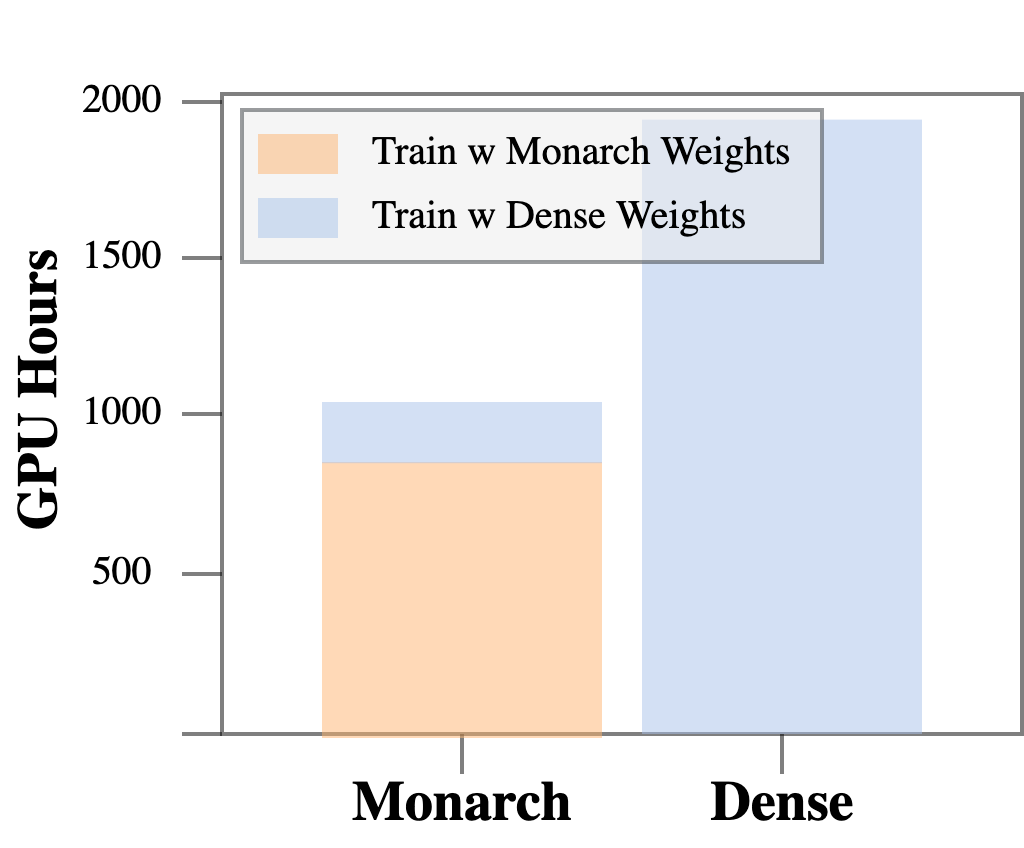
\includegraphics[width=.3\textwidth]{figures/rv_bar_temp.png}
  \vspace{-3mm}
  \caption{\label{fig:reverse_sparsification_bar}Time required (in A100 GPU hours) to reach the same perplexity (18.0)
    for GPT-2-small on OpenWebText.
    With ``reverse sparsification'', Monarch can speed up
    GPT-2 training by 2$\times$.\vspace{-1em}}
\end{figure}

We show that our Monarch approximation algorithm allows us to efficiently use
pretrained models, such as speeding up BERT finetuning on GLUE.

\paragraph{BERT finetuning.}
We take the BERT pretrained weights, approximate them with Monarch matrices,
and finetune the resulting model on the 9 GLUE tasks.
The results in \cref{table:bert_glue} shows that we obtain a Monarch finetuned
model with similar quality to the dense BERT model, but with 1.7$\times$ faster
finetuning speed.
This serves as a proof of concept, and we expect further speedup if additional model compression techniques are applied (e.g., quantization, kernel fusion).




\begin{table}[h]
  \small
  \centering
  \vspace{-5mm}
  \caption{\label{table:bert_glue}The performance of Monarch matrices in
    finetuning BERT on GLUE.}
  \setlength{\tabcolsep}{5pt}
  \vspace{1em}
  \iftoggle{arxiv}{}{
    \resizebox{\linewidth}{!}
  }
  {
  \begin{tabular}{@{}c||ccccccc@{}}
  \specialrule{.15em}{.05em}{.05em}
    Model&\multicolumn{1}{c}{GLUE (avg)}&\multicolumn{1}{c}{Speedup} &\multicolumn{1}{c}{Params} & \multicolumn{1}{c}{FLOPs} \\
    \specialrule{.15em}{.05em}{.05em}
    BERT-base & 78.6& - & 109M & 11.2G \\
    Monarch-BERT-base& 78.3& 1.5$\times$ & 55M & 6.2G  \\
    BERT-large & 80.4 & - & 335M & 39.5G \\
    Monarch-BERT-large & 79.6 & 1.7$\times$ & 144M & 14.6G  \\
    \specialrule{.15em}{.05em}{.05em}
  \end{tabular}
  }
  \vspace{-3mm}
\end{table}






\section{Related Work}


% \paragraph{Multilingual LLMs} Early work on large language models has mostly focused on English~\cite{brown2020language}. However, there has been a surge in multilingual models and accompanying datasets to address the need to use these models in non-English languages.

\textbf{Expanding Multilingual Language Models.} Initially, the development of LLMs has predominantly targeted the English language~\citep{brown2020language}, leveraging the extensive corpus of English data available on the Web and the broad applicability of models trained on English text. However, this emphasis has often come at the cost of accommodating the linguistic diversity found across various language demographics~\citep{zhu2023extrapolating,bang2023multitask,zhang2024m3exam}. Recognizing this significant limitation~\citep{robinson2023chatgpt,peng-etal-2024-humaneval}, recent research has proposed foundational LLMs equipped with multilingual capabilities~\citep{chai2023ernie, scao2022bloom,wei2023polylm,shliazhko2022mgpt}, or has explicitly concentrated on addressing the challenges posed by low-resource languages~\citep{ustun2024aya,singh2024aya,gala2023indictrans2}. To integrate multilingual capabilities into existing LLMs, researchers have proposed a variety of methods to enhance multilingual adaptation. These approaches range from continual pretraining techniques~\citep{ibrahim2024simple,gupta2023continual} to initial training on extensive multilingual datasets~\citep{scao2022bloom,chai2023ernie} and then subsequent specialized fine-tuning on a target language~\citep{yang2023bigtranslate, han-etal-2022-x}, and even adaptation through instruction tuning~\citep{shaham2024multilingual,kew2023turning,gala2024airavata}. Critical aspects in multilingual adaptation remain on the availability of high-quality diverse multilingual corpus~\citep{correa2024teenytinyllama} and further the scope of vocabulary of the specific language.

% \SVX{need to clearly state the difference from BLOOM and ERNIE-Code, LLMs on both multilingual NLs and multilingual code}

\textbf{Continual Pretraining.}  Static datasets are impractical for adapting to evolving real-world data, making continual learning essential~\citep{ring1998child,thrun1998lifelong}. Continual pretraining~\citep{gururangan2020dont} allows models to incorporate new knowledge without retraining from scratch, a costly endeavor. As curated datasets like RedPajama~\citep{together2023redpajama} and Dolma~\citep{soldaini2024dolma} become available, integrating them efficiently is crucial. This also enables the extension of models to new modalities, such as code (e.g., StableCode). Previous approaches focus on replay techniques, optimizing learning schedules~\citep{ibrahim2024simple}, soft masking~\citep{ke2023adapting}, and forward/backward transfer~\citep{yildiz2024investigating}.

% The notion of large static datasets becomes impractical when confronted with the dynamic nature of real-time events, evolving facts, and the introduction of new data or concepts within a domain. In such scenarios, continual learning~\citep{ring1998child,thrun1998lifelong,Kirkpatrick2018overcoming,zenke2017continual,rebuffi2017icarl,lopez2017gradient} becomes imperative for large pretrained models to swiftly adapt to these shifting environments. The drive for continual pretraining~\citep{gururangan2020dont} extends beyond the dynamic nature of real-world data; it is also fueled by the prohibitive expense associated with training current foundation models from scratch. As more curated datasets become accessible (e.g. RedPajama~\citep{together2023redpajama}, Dolma~\citep{soldaini2024dolma}, CommonCorpus\footnote{\url{https://huggingface.co/blog/Pclanglais/common-corpus}}, ToolQA~\citep{zhuang2023toolqa}) the idea of incorporating knowledge from these datasets through retraining on the union of all available data sets becomes inherently unfeasible. This also encompasses the integration of new capabilities into foundational models trained on specific data distributions. For example, it involves expanding natural language-based models to include the structured modality of code (e.g. StableCode\footnote{\url{https://stability.ai/news/stable-code-2024-llm-code-completion-release}}). Previous studies on continual pretraining have primarily concentrated on replay, optimizing the learning rate schedule~\citep{ibrahim2024simple}, preserving general knowledge through soft masking attention heads~\citep{ke2023adapting}, exploring the effects of domain similarity and model capacity on forward and backward transfer~\citep{yildiz2024investigating}, and continual post-training for few-shot adaptation~\citep{ke2022continual}.

% \citep{scao2022bloom}
% \citep{chai2023ernie}
% \citep{ustun2024aya}
% \citep{lin2021few}
% \citep{muennighoff2022crosslingual}
% \citep{shliazhko2022mgpt}
% \citep{scao2022language}

% \citep{singh2024aya}
% \citep{kudugunta2024madlad}
% \citep{longpre2023data}
% \citep{laurenccon2022bigscience}
% \citep{albalak2024survey}
% \citep{nguyen2023culturax}

% \textbf{LLM Compliance}
% The extensive utilization of Large Language Models (LLMs) across various applications underscores the necessity for their operation to uphold user privacy, mitigate risks such as misinformation or biased outputs, and ensure transparency regarding their functionality and utilization, all while adhering to local regulations. Independent evaluations and red teaming play crucial roles in assessing these risks. However, conflicts of interest within major AI companies may impede such safety evaluations, underscoring the necessity for a safe harbor for safety research~\citep{longpre2024safe}. Benchmark datasets facilitating such research efforts include those proposed by \cite{zhang2023safetybench} and \cite{sun2023safety}. Studies aimed at enhancing the security, safety, and legal compliance of Large Language Models (LLMs) have encompassed various approaches. These include the creation of datasets based on FAIR data principles~\citep{raza2024fair}, the development of structured LLM auditing mechanisms~\citep{M_kander_2023}, risk assessment of LLM alignment through personalized feedback~\citep{kirk2023personalisation}, structured evaluation of risks associated with LLM deployment~\citep{derczynski2023assessing}, and profiling foundation model transparency~\citep{bommasani2023foundation,bommasani2024foundation}.


\section{Conclusion}
% We have presented \system - an important contribution in the development of open-source, lawful, and accessible artificial intelligence. It demonstrates impressive multilingual and coding capabilities, along with a unique emphasis on aligning with safety guidelines outlined in the Biden-Harris US Executive Order on AI. \system posses several advantages: (1) it exemplifies the power of collaboration within the open-source community, promoting transparency and accessibility in AI development; (2) the model's ability to handle diverse languages, coding, and specialized domains showcases a broadening of AI utility for various applications; (3) the focus on red-teaming the model according to the Biden-Harris Executive Order underscores the importance of responsible AI development, ensuring alignment with government standards; and (4) the balance between safety, helpfulness, and state-of-the-art performance makes \system a valuable tool for researchers and developers. 



In this work, we introduced \textsc{\system}, a multilingual model that extends the capabilities of code-focused LLMs while maintaining their original coding proficiency. We demonstrate that continual training from code to multilingual tasks is feasible, allowing the model to perform well across both domains. Adhering to the safety guidelines of the Biden-Harris US Executive Order on AI, \textsc{\system} promotes responsible AI development while pushing the boundaries of performance and utility. Our two-stage continual pretraining approach, combined with insights from cross-lingual red-teaming, highlights the adaptability and versatility of modern language models. \textsc{\system} serves as a valuable resource for both researchers and developers, fostering collaboration and transparency in the open-source AI community. Future work will explore continual pretraining on stronger base models with the same two-stage curriculum, focusing on safety for both LLMs and Multimodal-LLMs. We also aim to develop domain-specific expert models, enhancing task specialization and expanding model versatility.







% We introduce \textsc{\system}, designed to align with legal standards and enhance accessibility. This model showcases proficiency in multilingual understanding and coding tasks, while prioritizing compliance with the safety guidelines outlined in the Biden-Harris US Executive Order on AI. Moreover, \textsc{\system}  exemplifies the collaborative nature of the open-source community, promoting transparency and accessibility in AI development. By red-teaming the model in accordance with the Biden-Harris Executive Order, it underscores the significance of responsible AI development and ensures alignment with government standards. Striking a balance between safety, utility, and cutting-edge performance, \textsc{\system} emerges as a valuable tool for researchers and developers. In addition, we present intriguing insights into cross-lingual red-teaming effects and emphasize the importance of the two-stage curriculum-based continual pretraining approach. 

% \paragraph{Future Work.}
% Leveraging insights from \system's development, we plan to explore continual pretraining of stronger base models using the same two-stage curriculum, prioritizing safety. This applies to both LLMs and Multimodal-LLMs (MLLMs). Furthermore, we aim to train multiple independent domain experts based on \system, potentially merging them to improve task specialization.


% \newpage

\section*{Ethical Consideration}
We believe that transparency and accessibility are fundamental principles in the development and deployment of artificial intelligence technologies. Closed-source LLMs limit public scrutiny, hinder collaboration, and potentially reinforce biases inherent in their development process. 
In contrast, our commitment to open source models fosters a culture of accountability, collaboration, and inclusivity. By making \system\ accessible to all, we promote innovation, empower diverse voices, and strive for equitable outcomes in AI applications. We firmly believe that openness in AI development is essential for creating solutions that truly serve the needs and values of society. To this end, we prioritized safety guardrails in alignment with the Biden-Harris Executive Order on AI. Furthermore, the multilingual capability of \system\ enhances its usability for users across the world.

On the other hand, each promise comes with peril, and improved technological access through \system\ might also increase the potential number of malicious actors. We overall believe that the general benefit far outweighs the potential misuse and want to emphasize the importance of a considered and ethical use of this technology and thus also of \system.

Lastly, we recognize that safety and lawfulness can be contextual to different cultures and laws. We recognize that in our work we focused on a U.S. centric standard, and we believe future work should also explore multi-jurisdictional redteaming.


\section*{Acknowledgments}
This work was supported by the ``R\&D Hub Aimed at Ensuring Transparency and Reliability of Generative AI Models'' project of the Ministry of Education, Culture, Sports, Science and Technology, and used resources of LUMI supercomputer under project\_462000316.

% This document has been adapted by Emily Allaway from the instructions for earlier ACL and NAACL proceedings, including those for NAACL 2024 by Steven Bethard, Ryan Cotterell and Rui Yan,
% ACL 2019 by Douwe Kiela and Ivan Vuli\'{c},
% NAACL 2019 by Stephanie Lukin and Alla Roskovskaya,
% ACL 2018 by Shay Cohen, Kevin Gimpel, and Wei Lu,
% NAACL 2018 by Margaret Mitchell and Stephanie Lukin,
% Bib\TeX{} suggestions for (NA)ACL 2017/2018 from Jason Eisner,
% ACL 2017 by Dan Gildea and Min-Yen Kan,
% NAACL 2017 by Margaret Mitchell,
% ACL 2012 by Maggie Li and Michael White,
% ACL 2010 by Jing-Shin Chang and Philipp Koehn,
% ACL 2008 by Johanna D. Moore, Simone Teufel, James Allan, and Sadaoki Furui,
% ACL 2005 by Hwee Tou Ng and Kemal Oflazer,
% ACL 2002 by Eugene Charniak and Dekang Lin,
% and earlier ACL and EACL formats written by several people, including
% John Chen, Henry S. Thompson and Donald Walker.
% Additional elements were taken from the formatting instructions of the \emph{International Joint Conference on Artificial Intelligence} and the \emph{Conference on Computer Vision and Pattern Recognition}.

% % Bibliography entries for the entire Anthology, followed by custom entries
% \bibliography{anthology,custom}
% % Custom bibliography entries only
\bibliography{custom}

\appendix

\appendix

% \section{Claimed Emergent Abilities}
% \label{app:claimed_emergent_abilities}

% We compile the models, tasks and metrics that different papers have claimed reveal emergent abilities of large language models. This list may be incomplete or inaccurate, but represents a good faith attempt to compile this information. Note: quantifying model scale when an ability emerges is complicated by the fact that different papers report model scale differently, either as (a) number of parameters \cite{brown2020language, ganguli2022predictability}, (b) effective number of parameters \cite{srivastava2022beyond} or (c) training FLOPs \cite{wei2022emergent}.

% \begin{table}[h!]
%     \centering
%     \begin{tabular}{|l|c|c|c|}
%     \hline
%         Task & Model Families & Metric & Model Scale at Emergence \\
%         \hline
%         2-Digit Addition \cite{brown2020language} & GPT-3 & Accuracy & 13B Parameters\\
%         2-Digit Subtraction \cite{brown2020language} & GPT-3 & Accuracy & 13B Parameters\\
%         3-Digit Addition \cite{brown2020language, ganguli2022predictability} & GPT-3 & Accuracy & 175B Parameters\\
%         3-Digit Subtraction \cite{brown2020language} & GPT-3 & Accuracy & 175B Parameters\\
%         MMLU \cite{ganguli2022predictability} & GPT-3, Gopher & Accuracy & 200B, 300B Parameters\\
%         Program Synthesis \cite{ganguli2022predictability} & Google Internal & \% Samples Solving Task & 200B Parameters\\
%         Figure of Speech Detection \cite{srivastava2022beyond} & ? & ? & $\sim 10^{11}$ Effective Parameters \\
%         IPA Transliterate \cite{srivastava2022beyond, wei2022emergent} & LaMDA, GPT-3 & BLEU & $\sim 10^{23}, \sim 10^{23}$ Training FLOPs\\
%         Periodic Elements \cite{srivastava2022beyond} & ? & ? & ?\\
%         Modified Arithmetic \cite{srivastava2022beyond, wei2022emergent} & GPT-3, LaMDA & Accuracy & $\sim 10^{23}, \sim 10^{24}$ Training FLOPs\\
%         Repeat Copy Logic \cite{srivastava2022beyond} & ? & ? & $10^{11}$ Effective Parameters\\
%         Word Unscrambling \cite{srivastava2022beyond, wei2022emergent} & LaMDA & Exact Match & $\sim 10^{24}$ Training FLOPs\\
%         Persian QA \cite{wei2022emergent} & PaLM & Exact Match & $\sim 10^{24}$ Training FLOPs\\
%         Truthful QA \cite{wei2022emergent} & Gopher & Accuracy & $\sim 10^{23}$ Training FLOPs\\
%         Grounded Mappings \cite{wei2022emergent} & ? & ? & ?\\
%         Multi-task NLU \cite{wei2022emergent} & ? & ? & ?\\
%         Word in context \cite{wei2022emergent} & ? & ? & $\sim 10^{24}$ Training FLOPs\\
%         \hline
%     \end{tabular}
%     \newline
%     \caption{\textbf{Tasks, model families, metrics and number of parameters for emergent abilities.}}
%     \label{tab:my_label}
% \end{table}


% \section{Exponentiated Negative Cross Entropy Lower Bounds Accuracy}
% \label{app:acc_bound}

% Consider batch size $B$ with length $L$. During training i.e. with teacher-forcing, the per-token accuracy (averaged over batch index $b$ and sequence index $l$) is defined as:
% %
% \begin{align}
%     \text{Acc} &\defeq \frac{1}{B} \sum_b \frac{1}{L} \sum_l p(t_{bl}^* | t_{b, <l}^*)\\
%     &= \frac{1}{BL} \sum_{b, l} p(t_{bl}^* | t_{b, <l}^*)
% \end{align}

% The cross entropy (commonly averaged over the batch) is defined as:
% %
% \begin{align}
%     \mathcal{L}_{CE} &\defeq -\frac{1}{B} \sum_b \log p(t_{b 1}^*, ..., t_{b L}^*)\\
%     &= -\frac{1}{B} \sum_b \log \prod_l p(t_{b l}^*| t_{b, <l}^*)\\
%     &= -\frac{1}{B} \sum_{b, l} \log p(t_{bl}^* | t_{b, <l}^*)
% \end{align}

% To make the comparison between accuracy and cross entropy a little easier, let's normalize the cross entropy by the sequence length:
% %
% \begin{align}
%     \mathcal{L}_{CE/L} &\defeq \frac{1}{L}\mathcal{L}_{CE}\\
%     &=  -\frac{1}{BL} \sum_{b, l} \log p(t_{bl}^* | t_{b, <l}^*)
% \end{align}

% Recall that Jensen's inequality tells us that for any random variable $X$, $\log \mathbb{E}[X] \geq \mathbb{E}[\log X]$. The relationship between sequence-length-normalized cross entropy and accuracy is thus:
% %
% \begin{align}
%     -\mathcal{L}_{CE/L} = \frac{1}{BL} \sum_{b, l} \log p(t_{bl}^* | t_{b <l}^*) &\leq \log \frac{1}{BL} \sum_{b, l}  p(t_{bl}^* | t_{b <l}^*) = \log \text{Acc}\\
%     \exp(- \mathcal{L}_{CE/L}) &\leq \text{Acc}
% \end{align}

% Consequently, we see that driving the cross entropy loss to $0$ necessarily drives the accuracy to $1$.

% TODO: Can we use the second moment method to derive bounds on how (un)likely a subset of tokens are to deviate from the mean?


\section{Approximate Behavior of Metrics on Sequential Data}
\label{app:metric_scaling}

How do different metrics behave when used to measure autoregressive model outputs? Precisely answering this question is tricky and possibly analytically unsolvable, so we provide an approximate answer here.

Notationally, we consider $N$ test data of length $L$ (here, length is measured in tokens) with targets denoted $t_n \defeq (t_{n1}, t_{n2}, ... t_{nL})$, the autoregressive model has a true-but-unknown per-token error probability of $\epsilon \in [0, 1]$ and the model outputs prediction $\hat{t}_n \defeq (\hat{t}_{n1}, \hat{t}_{n2}, ... \hat{t}_{nL})$. This assumes that the model's per-token error probability is constant, which is empirically false, but modeling the complex dependencies of errors is beyond our scope.

\subsection{Per-Token Error Probability is Resolution-Limited}
\label{app:metric_scaling:resolution_limited}

Note that because we have $N$ test data, each of length $L$, our resolution for viewing the per-token error probability $\epsilon$ is limited by $1/NL$. 
Here, resolution refers to ``the smallest interval measurable by a scientific instrument; the resolving power."
To explain what resolution means via an example, suppose one wants to measure a coin's probability of yielding heads.
After a single coin flip, only two outcomes are possible (H, T), so the resolution-limited probability of heads is either $0$ or $1$.
After two coin flips, four outcomes are possible (HH, HT, TH, TT), so the resolution-limited probability of heads is now one of $0, 0.5, 1$.
After $F$ coin flips, we can only resolve the coin's probability of yielding heads up to $1/F$.
Consequently, we introduce a resolution-limited notation:
%
\begin{equation}
    \nint{a}_b \defeq \text{$a$ rounded to the nearest integer multiple of $1/b$}
\end{equation}

\subsection{Token Edit Distance}
\label{app:metric_scaling:token_edit_distance}

We first consider an adaptation of the Levenshtein (string edit) distance for models that function on tokens rather than characters, an adaptation we term the \textit{token edit distance}. The token edit distance between two token sequences $t_n, \hat{t_n}$ is defined as the integer number of additions, deletions or substitutions necessary to transform $t_n$ into $\hat{t}_n$ (or vice versa).

\begin{align}
    \text{Token Edit Distance}(t_n, \hat{t}_n)  &\defeq \text{Num Substitutions} + \text{Num. Additions} + \text{Num. Deletions}\\
    &= \sum_{\ell =1}^L \mathbb{I}[t_{n\ell} \neq \hat{t}_{n\ell}] + \text{Num. Additions} + \text{Num. Deletions}\\
    &\geq \sum_{\ell =1}^L \mathbb{I}[t_{n\ell} \neq \hat{t}_{n\ell}]
\end{align}

The expected token edit distance is therefore:

\begin{align}
    \mathbb{E}[\text{Token Edit Distance}(t_n, \hat{t}_n)] &\geq \mathbb{E}[\sum_{\ell =1}^L \mathbb{I}[t_{n\ell} \neq \hat{t}_{n\ell}]]\\
    &= \sum_{\ell =1}^L p(t_{n\ell} \neq \hat{t}_{n\ell})\\
    &\approx L (1 - \epsilon)
\end{align}

The resolution-limited expected token edit distance is therefore:

\begin{equation}
    \nint{\mathbb{E}[\text{Token Edit Distance}(t_n, \hat{t}_n)]}_{NL} \geq L \Big(1 - \nint{\epsilon}_{NL} \Big)
\end{equation}

From this, we see that the expected token edit distance scales approximately linearly with the resolution-limited per-token probability. The real rate is slightly higher than linear because additions and deletions contribute an additional non-negative cost, but modeling this requires a model of how likely the model is to overproduce or underproduce tokens, which is something we do not currently possess.

\subsection{Accuracy}
\label{app:metric_scaling:accuracy}

\begin{align}
    \text{Accuracy}(t_n, \hat{t}_n) &\defeq \mathbb{I}[\text{No additions}] \, \mathbb{I}[\text{No deletions}] \, \prod_{l=1}^L \mathbb{I}[t_{nl} = \hat{t}_{nl}]\\
    &\approx \prod_{l=1}^L \mathbb{I}[t_{nl} = \hat{t}_{nl}]
\end{align}

As with the Token Edit Distance (App. \ref{app:metric_scaling:accuracy}), we ignore how likely the language model is to overproduce or underproduce tokens because we do not have a good model of this process. Continuing along,

\begin{align}
    \mathbb{E}[\log \text{Accuracy}] &= \sum_l \mathbb{E}[\log \mathbb{I}[t_{nl} = \hat{t}_{nl}]]\\
    &\leq \sum_l \log \mathbb{E}[\mathbb{I}[t_{nl} = \hat{t}_{nl}]]\\
    &\approx L \log (1- \epsilon)
    % \exp(\mathbb{E}[\log \text{Accuracy}]) &= \exp (\sum_l \mathbb{E}[\log \mathbb{I}(t_{nl}, \hat{t}_{nl})])\\
    % &=
\end{align}

Taking an approximation that would make most mathematicians cry:

\begin{align}
    \mathbb{E}[\text{Accuracy}] &\approx \exp(\mathbb{E}[\log \text{Accuracy}])\\
    &= (1 - \epsilon)^L\\
\end{align}

This reveals that accuracy \textbf{approximately} falls geometrically with target token length. The resolution-limited expected accuracy is therefore:

\begin{equation}
    \nint{\mathbb{E}[\text{Accuracy}]}_{NL} = \nint{(1 - \epsilon)^L}_{NL}
\end{equation}

From this we can see that choosing a nonlinear metric like Accuracy is affected significantly more by limited resolution because Accuracy forces one to distinguish quantities that decay rapidly.

\subsection{ROUGE-L-Sum}
\label{app:metric_scaling:rougeLsum}

\begin{figure}
    \centering
    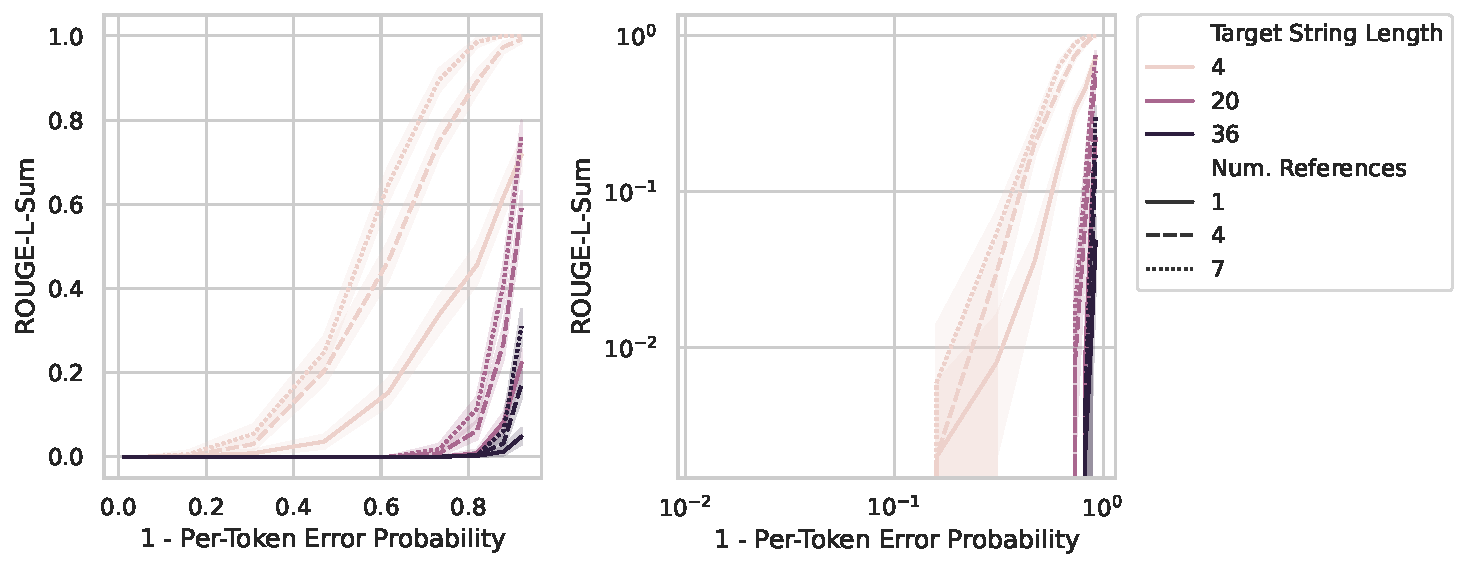
\includegraphics[width=0.95\textwidth]{figures/rouge_understanding/rougeLsum_vs_token_error_prob_scaling_simulation.pdf}
    \caption{\textbf{ROUGE-L-Sum is a sharp metric.} Simulations show that as the per-token error probability slightly increase (e.g. from 0.05 to 0.1), the ROUGE-L-Sum metric sharply falls.}
    \label{fig:app:metric_scaling:rougeLsum}
\end{figure}


Another BIG-Bench metric \cite{srivastava2022beyond} is ROUGE-L-Sum \cite{lin2004rouge}, a metric based on the longest common subsequence (LCS) between two sequences. Section 3.2 of \cite{lin2004rouge} gives the exact definition, but the key property is that ROUGE-L-Sum measures the ``union" LCS, which means ``stitching" together LCSs across the candidate and multiple references. As explained in the original paper: if the candidate sequence is $c = w_1 w_2 w_3 w_4 w_5$, and if there are two reference sequences $r_1 = w_1 w_2 w_6 w_7 w_8$ and $r_2 = w_1 w_3 w_8 w_9 w_5$, then $LCS(r_1, c) = w_1 w_2$ and $LCS(r_2, c) =w_1 w_3 w_5$, then the \textit{union} 
-LCS of $c, r_1, r_2$ is $w_1 w_2 w_3 w_5$, with length 4. Intuitively, this disproportionately benefits models with smaller error rates because their mistakes can be ``stitched" across multiple references; this is confirmed in simulation (Fig. \ref{fig:app:metric_scaling:rougeLsum}).


% \subsection{BLEU}
% \label{app:metric_scaling:bleu}


% \subsection{Emergence does not require on scaling laws: decreasing cross-entropy loss and stricter exact match is all you need }

% The goal of this section is to show that scaling laws are not necessary to create emergence and that many functional forms of the loss are valid as long as the form decreases as some other variable decreases -- say the number of parameters in the model.
% This typically holds in modern machine learning. 
% We do this by considering different functional forms of the cross entropy $CE(N)$, as a function of the number of parameters $N$, and show emergence, i.e. sharpness and unpredictability.
% We illustrate this by showing the programmer can exaggerate the sharpness (and therefore emergence) by implying increasing the exact number of tokens required to get correct in the accuracy, i.e. increasing $L$ in our notation.

% \subsubsection{Argument}

% Recall from section \ref{sec:alt_explanation} the accuracy requiring all $L$ tokens to be correct for a model of size $N$ as a function of cross-entropy $CE(N)$:

% \begin{equation*}
%     \text{Accuracy}(N) \approx p_N(\text{single token correct})^{\text{num. of tokens}} = \exp \Big(- CE(N) \Big)^L
% \end{equation*}

% We plot this equation using three functional forms for a decreasing cross-entropy loss in figure \ref{fig:decreasing_loss_leads_to_emergence_as_L_increases} for increasing values of $L$.
% These increasing values of $L$ induce a sharper -- therefore, seemingly more emergent curve when plotting the accuracy. 
% This means that if the programmer simply requires a stricter accuracy, he can make a perfectly smooth and predictable cross-entropy loss suddenly become sharp and unpredictable, i.e. ``emergent". 
% We show numerically it is independent of the functional form and instead that it only requires the cross-entropy to be decreasing and the accuracy metric to have some non-linear transformation that makes it sharper. 
% Therefore, if one had only tracked the cross-entropy loss instead, one could have had a smooth predictable curve for the models.
% This implies small-scale experimentation is still relevant, and we wish to highly that GPT-4 \cite{gpt4} small-scale experiment in conjunction with scaling loss. 
% We'd like to emphasize that changing the evaluation metric can suddenly induce emergence, and it is not an intrinsic property of the model. 

% %The goal will be to show that if $CE(N)$ decreases with different functional forms that $acc$ is emergent (either sharp or unpredictable).
% % TODO: sharp due to L
% % TODO: unpredictable due to constant and L

% \begin{figure}[htbp]
%   \centering
%   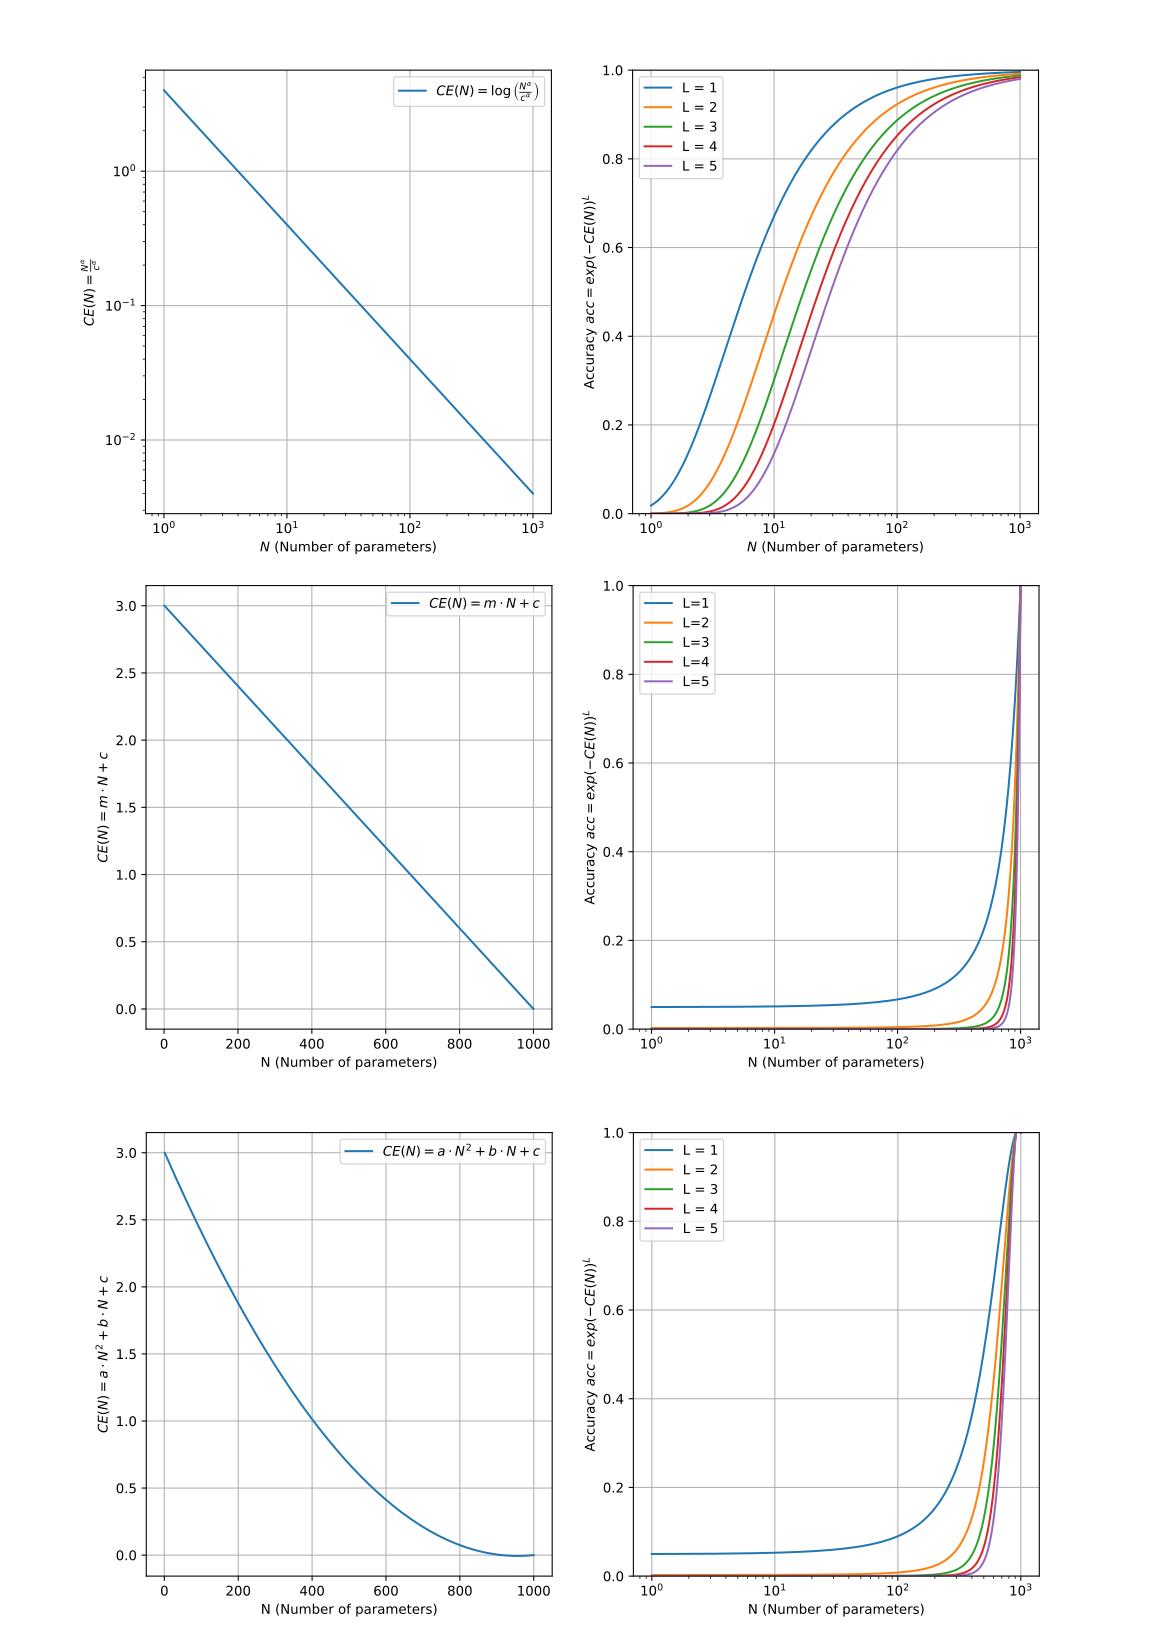
\includegraphics[width=0.8\textwidth]{figures/loss_decreasing_leads_to_emergence/decreasing_loss_leads_to_emergence_as_L_increases.png}
%   \caption{
%   \textbf{Emergence does not depend on scaling laws: any decreasing cross-entropy loss induces apparent emergence as L increases as you require more tokens to be exactly correct, i.e. L increases.}
%   The first row shows the same argument as in the main section, where a decreasing cross-entropy loss as a scaling law induces emergence as $L$ increases.
%   The second row shows the that apparent emergence is induced even when the cross-entropy loss decreases linearly.
%   The third row shows that the apparent emergence is induced when the cross-entropy loss decreases quadratically.
%   Emergence is amplified in this case especially by the increase in sharpness as more tokens are required to be correct. 
%   This means that simply changing the evaluation metric can suddenly induce emergence, and it is not an intrinsic property of the model. 
%   }
%   \label{fig:decreasing_loss_leads_to_emergence_as_L_increases}
% \end{figure}


\section{Inducing Emergent Abilities in Networks on Vision Tasks}
\label{app:sec:inducing_emergence_vision}

\subsection{Emergent Classification of MNIST Handwritten Digits by Convolutional Networks}

\begin{figure}
    \centering
    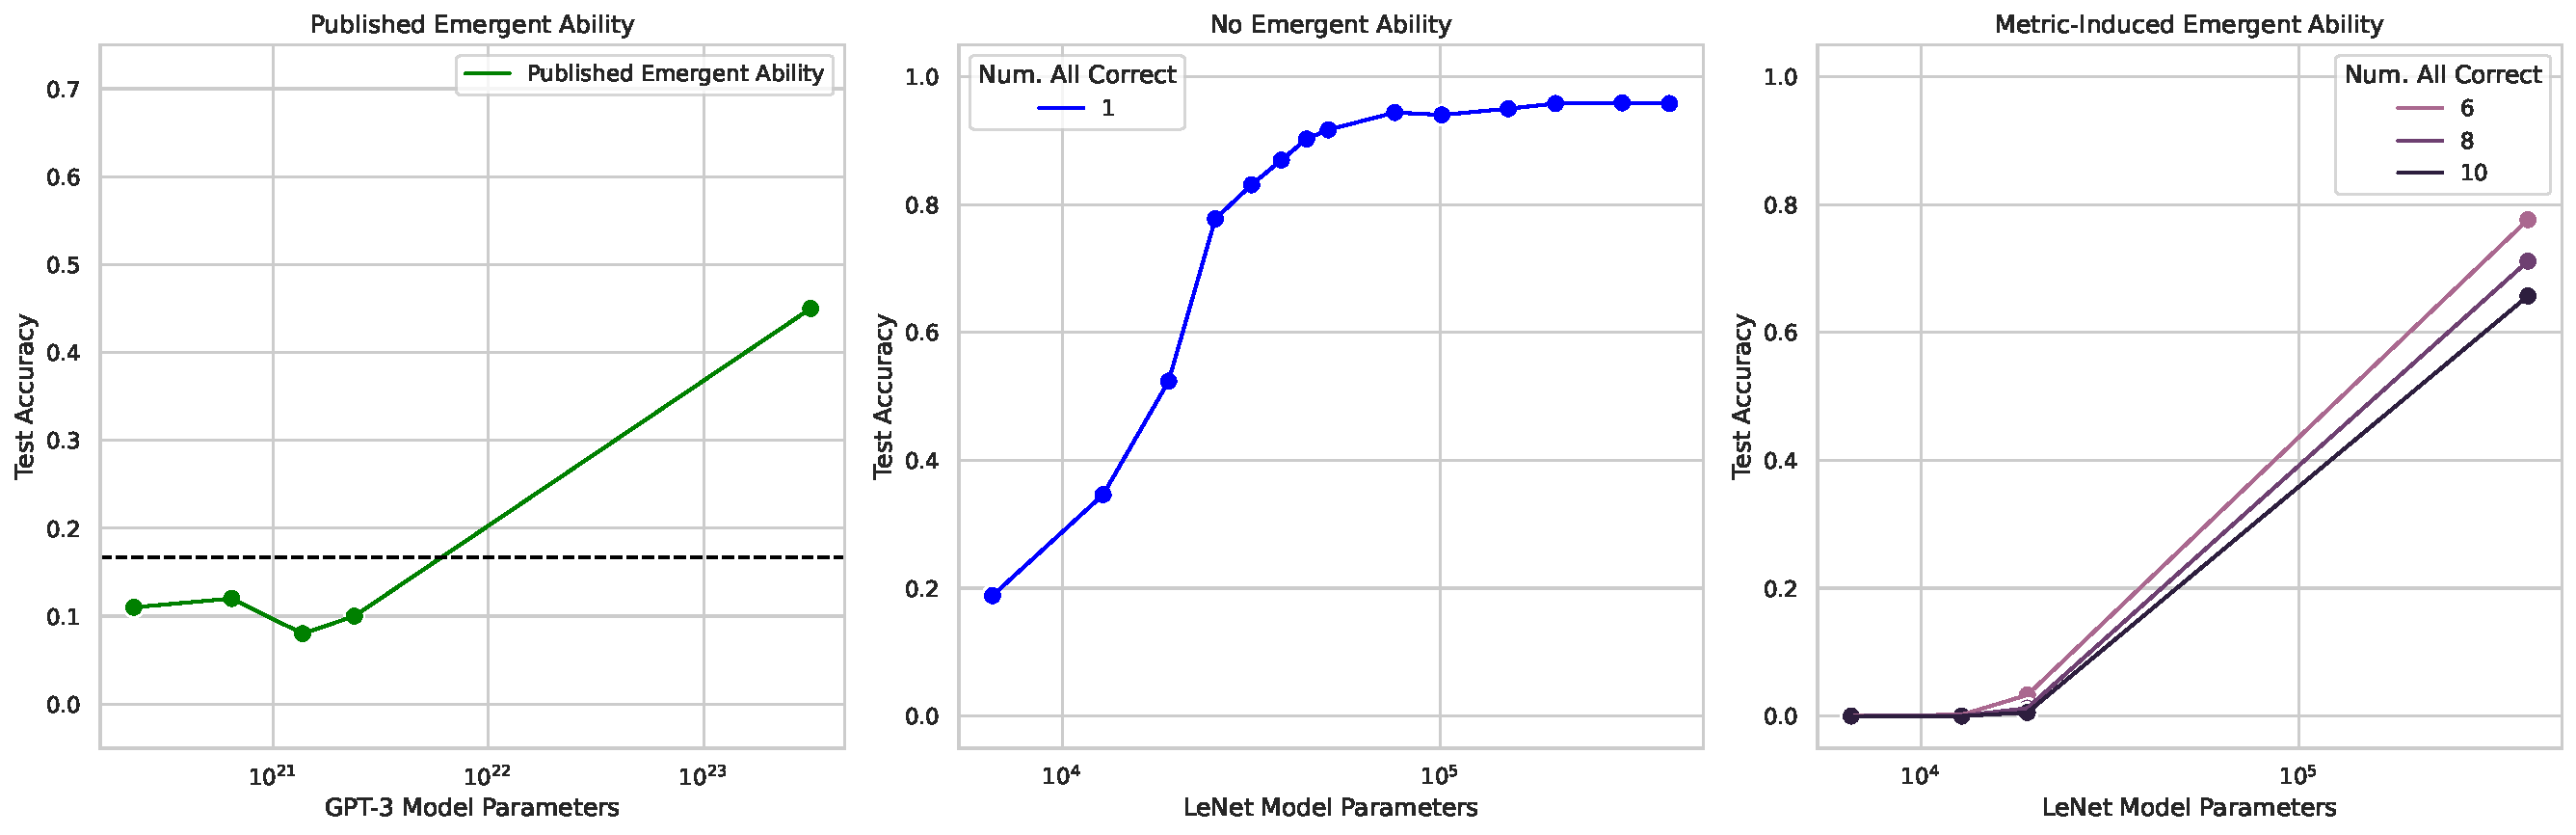
\includegraphics[width=\textwidth]{figures/vision/no_emergence_and_emergence_dataset=mnist.pdf}
    \caption{\textbf{Induced emergent MNIST classification ability in convolutional networks.} (A) A published emergent ability from the BIG-Bench Grounded Mappings task \cite{wei2022emergent}. (B) LeNet trained on MNIST \cite{lecun1998mnist} displays a predictable, commonplace sigmoidal increase in test accuracy as model parameters increase. (C) When accuracy is redefined as correctly classifying $K$ out of $K$ independent test data, this newly defined metric induces a seemingly unpredictable change.}
    \label{fig:vision_mnist}
\end{figure}

We begin by inducing an emergent classification ability in a LeNet convolutional neural network family \cite{lecun1998gradient}, trained on the MNIST handwritten digits dataset \cite{lecun1998mnist}.
This family displays smoothly increasing test accuracy as the number of parameters increase (Fig. \ref{fig:vision_mnist}B).
To emulate the accuracy metric used by emergence papers \cite{ganguli2022predictability, wei2022emergent, srivastava2022beyond}, we use \textit{subset accuracy}: 1 if the network classifies $K$ out of $K$ (independent) test data correctly, 0 otherwise.
Under this definition of accuracy, the model family displays an ``emergent" ability to correctly classify sets of MNIST digits as $K$ increases from $1$ to $5$, especially when combined with sparse sampling of model sizes (Fig. \ref{fig:vision_mnist}C).
This convolutional family's emergent classification ability qualitatively matches published emergent abilities, e.g., at the BIG-Bench Grounded Mappings task \cite{wei2022emergent} (Fig. \ref{fig:vision_mnist}A).




\end{document}
